\documentclass[a4paper]{report}
\usepackage[utf8]{inputenc}
\usepackage[portuguese]{babel}
\usepackage{hyperref}
\usepackage{a4wide}
\hypersetup{pdftitle={Trabalho 1},
pdfauthor={João Teixeira, José Ferreira, Maria Silva, Miguel Solino},
colorlinks=true,
urlcolor=blue,
linkcolor=black}
\usepackage{subcaption}
\usepackage[cache=false]{minted}
\usepackage{listings}
\usepackage{booktabs}
\usepackage{multirow}
\usepackage{appendix}
\usepackage{tikz}
\usepackage{authblk}
\usepackage{bashful}
\usepackage{verbatim}
\usepackage{amsmath}
\usetikzlibrary{positioning,automata,decorations.markings}

\begin{document}

\title{Fase 1\\ 
\large Grupo Nº 8}
\author{João Teixeira (A85504) \and José Ferreira (A83683) \and Maria Silva (A83840) \and Miguel Solino (A86435)}

\date{\today}

\begin{center}
    \begin{minipage}{0.75\linewidth}
        \centering
        
\includegraphics[width=0.4\textwidth]{images/eng.jpeg}\par\vspace{1cm}
        \vspace{1.5cm}
        \href{https://www.uminho.pt/PT}
        {\color{black}{\scshape\LARGE Universidade do Minho}} \par
        \vspace{1cm}
        \href{https://www.di.uminho.pt/}
        {\color{black}{\scshape\Large Departamento de Informática}} \par
        \vspace{1.5cm}
        \maketitle
    \end{minipage}
\end{center}

\tableofcontents

\pagebreak

\chapter{Introdução}

Este relatório tem como objetivo apresentar a fase inicial do projeto da Unidade
Curricular de Desenvolvimento de Sistemas de Software.\\
Ao longo deste relatório apresentamos as considerações tidas em conta pelo grupo
ao longo da elaboração e formulação dos vário modelos e diagramas propostos:
\begin{enumerate}
    \item Modelo de Domínio, modelo conceptual que contém os
        comportamentos e dados;
    \item Use Cases;
    \item Diagrama de Use Cases;
    \item Especificações dos mesmos.
\end{enumerate}
Por fim irá ser apresentado um \textit{mockup} do produto final.

\chapter{Modelo de Domínio}

O sistema a implementar deve suportar a gestão de media e utilização da mesma
para uma residência onde esteja instalado.\\
Neste capítulo são apresentados os requisitos do problema e uma proposta de 
Modelo de Domínio.

\section{Descrição do Modelo de Domínio}

O problema em questão consiste em desenvolver um sistema de gestão e streaming
de media.\\
Após analisar o enunciado disponibilizado, concluímos que era necessário a
existência de vários conceitos a incluir na modelação do problema: Utilizador,
Media (música e vídeo), Biblioteca de media, Caracterização (do media que for
adicionada ao sistema por um utilizador), Download/Upload de media, Conta,
Conexões (de amizades entre utilizadores, ou seja, uma lista de Amigos).\\
Com isto, foram definidas as relações entre os conceitos referidos em cima:
\begin{itemize}
    \item cada Utilizador só pode ter uma conta, só pode fazer download do
        media que fez upload e só pode classificar o media e bibliotecas
        que lhe pertencem;
    \item cada media/biblioteca de media pode ter uma ou mais classificações;
    \item cada conta tem só um email, nome e password associados;
    \item conta não é obrigatório para utilizar o sistema mas fica limitado 
        a só usufruir de media;
\end{itemize}
Os utilizadores não devem ter a permissão de criar contas, logo para um
utilizador ter uma conta precisa que algum outro com permissões de
administrador crie a conta sem password para mais tarde os utilizadores
das contas a definam.

\section{Modelo de Domínio}

\begin{figure}[H]
	\centering 
    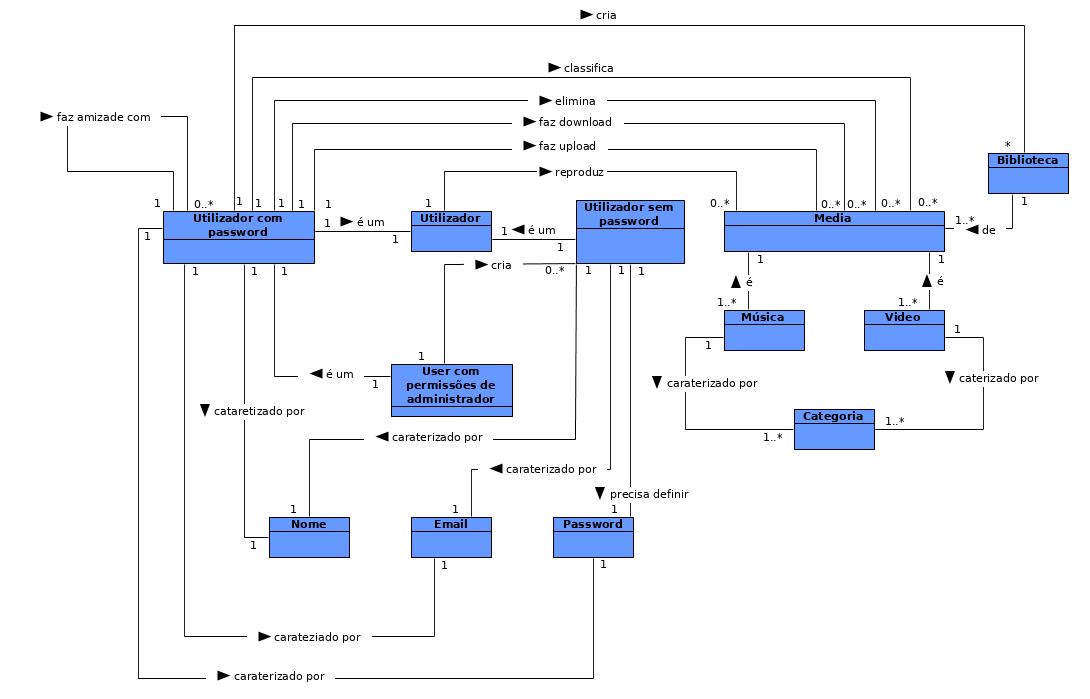
\includegraphics[width=\textwidth]{images/Dominio.png}  
    \caption{Modelo de Domínio}
\end{figure}


\chapter{Use Cases}

O Diagrama de Use Cases representa os atores do sistema e as tarefas de cada um
deles. No nosso caso existem 4 atores:
\begin{itemize}
    \item \textbf{Utilizador}: Todos os outros referidos abaixo são atores deste
        tipo. Logo, a este ator estará relacionado as ações que todos podem
        fazer
    \item \textbf{Utilizador sem password}: É um utilizador que após ter pedido
        a um administrador para lhe criar uma conta dando o email e nome, pode
        definir a sua password para passar a ser um utilizador com password
    \item \textbf{Utilizador com password}: Ter password significa que já tem
        uma conta "completa", ou seja, tem acesso à totalidade de ações que um
        user sem permissões de administrador pode ter
    \item \textbf{Utilizador com permissões de administrador}: A diferença deste 
        utilizador para os restantes é que este é o único que pode criar uma
        conta e assim ser o responsável pela existência dos restantes.
\end{itemize}

\begin{figure}[H]
	\centering 
    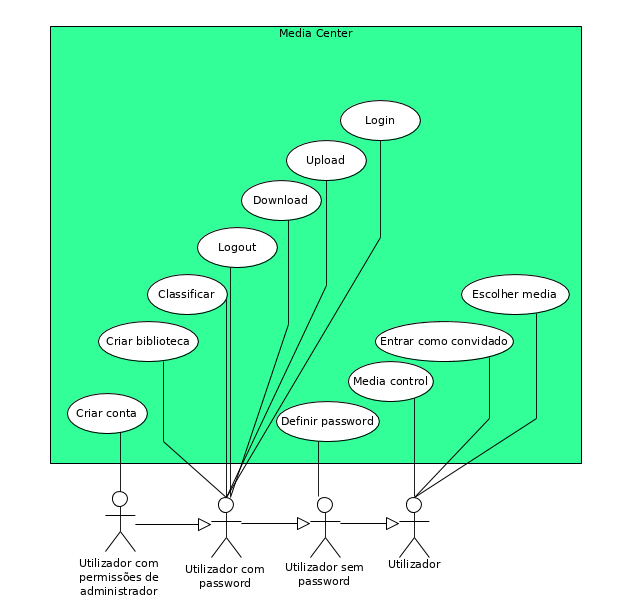
\includegraphics[width=\textwidth]{images/UseCases.png}  
    \caption{Diagrama de Use Cases}
\end{figure}



\section{Especificações dos Use Cases}

Nesta parte optamos por ordenar os use cases por permissões, ou seja, começamos
por apresentar os de um utilizador normal, seguido de um utilizador sem
password, utilizador com password e utilizador com permissões de administrador.

\subsection{Entrar como convidado}

\begin{figure}[H]
	\centering 
    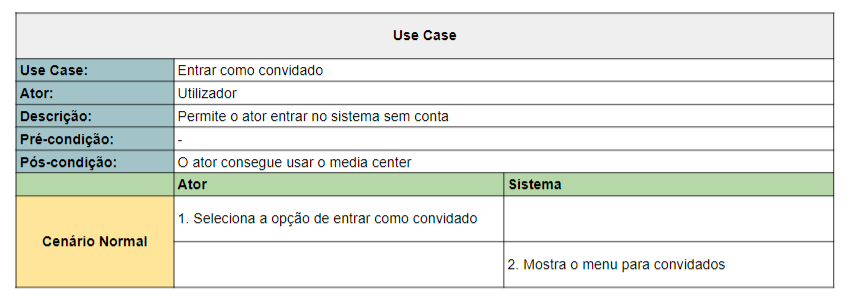
\includegraphics[width=\textwidth]{images/Entrar_como_convidado.png}  
    \caption{Especificação do \emph{Use Case} Entrar como convidado}
\end{figure}

\subsection{Media Control}

\begin{figure}[H]
	\centering 
    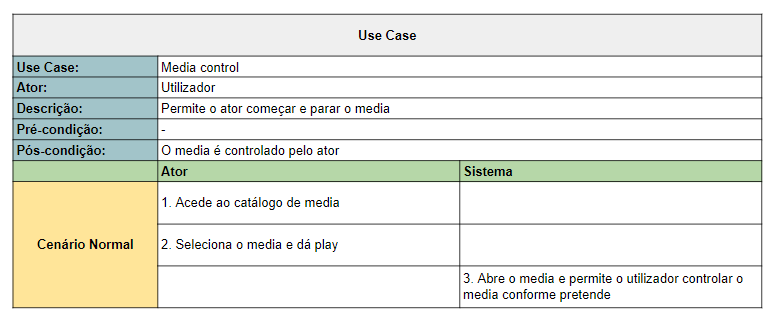
\includegraphics[width=\textwidth]{images/Media_Control.png}  
    \caption{Especificação do \emph{Use Case} Media Control}
\end{figure}

\subsection{Escolher media}

\begin{figure}[H]
	\centering 
    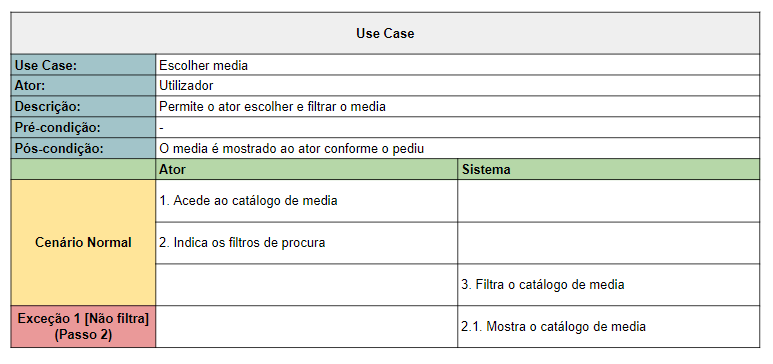
\includegraphics[width=\textwidth]{images/Escolher_Media.png}  
    \caption{Especificação do \emph{Use Case} Escolher media}
\end{figure}

\subsection{Definir password}

\begin{figure}[H]
	\centering 
    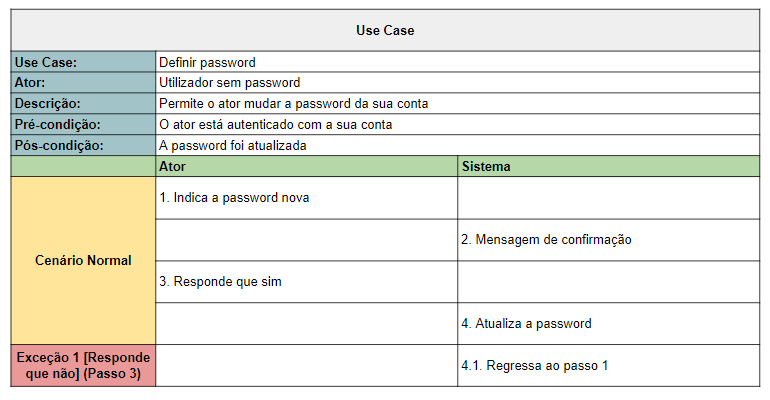
\includegraphics[width=\textwidth]{images/Definir_Password.png}  
    \caption{Especificação do \emph{Use Case} Definir password}
\end{figure}

\subsection{Login}

\begin{figure}[H]
	\centering 
    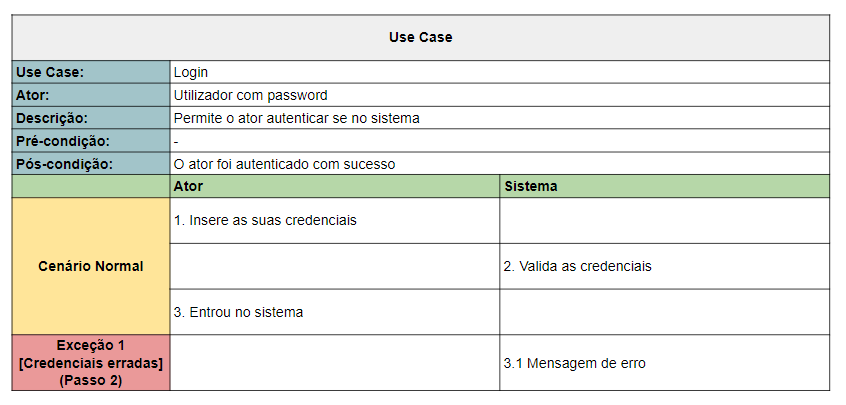
\includegraphics[width=\textwidth]{images/Login.png}  
	\caption{Especificação do \emph{Use Case} Login}
\end{figure}

\subsection{Logout}

\begin{figure}[H]
	\centering 
    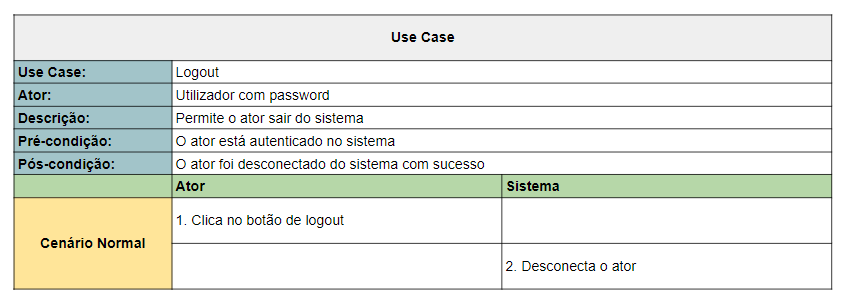
\includegraphics[width=\textwidth]{images/Logout.png}  
    \caption{Especificação do \emph{Use Case} Logout}
\end{figure}

\subsection{Download}

\begin{figure}[H]
	\centering 
    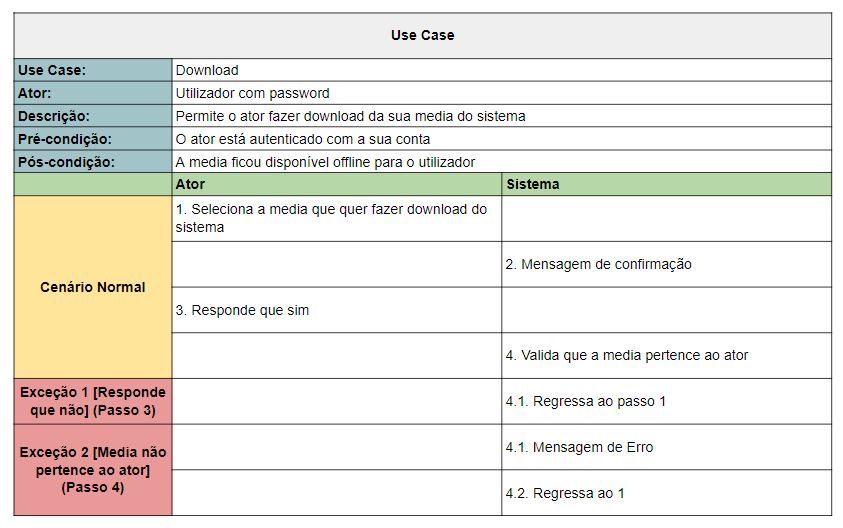
\includegraphics[width=\textwidth]{images/Download.png}  
    \caption{Especificação do \emph{Use Case} Download}
\end{figure}

\subsection{Upload}

\begin{figure}[h]
	\centering 
    \includegraphics[width=\textwidth]{images/upload.png}  
    \caption{especificação do \emph{use case} upload}
\end{figure}

\subsection{Eliminar media}

\begin{figure}[h]
	\centering 
    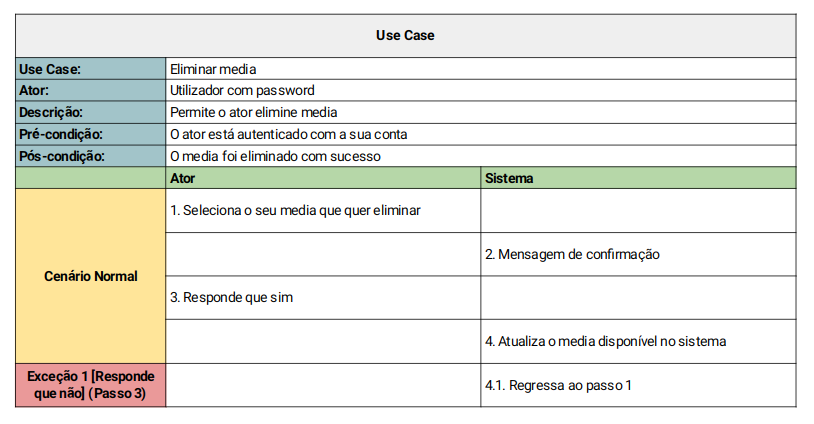
\includegraphics[width=\textwidth]{images/Eliminar_media.png}  
    \caption{especificação do \emph{use case} Eliminar media}
\end{figure}

\subsection{Classificar}

\begin{figure}[H]
	\centering 
    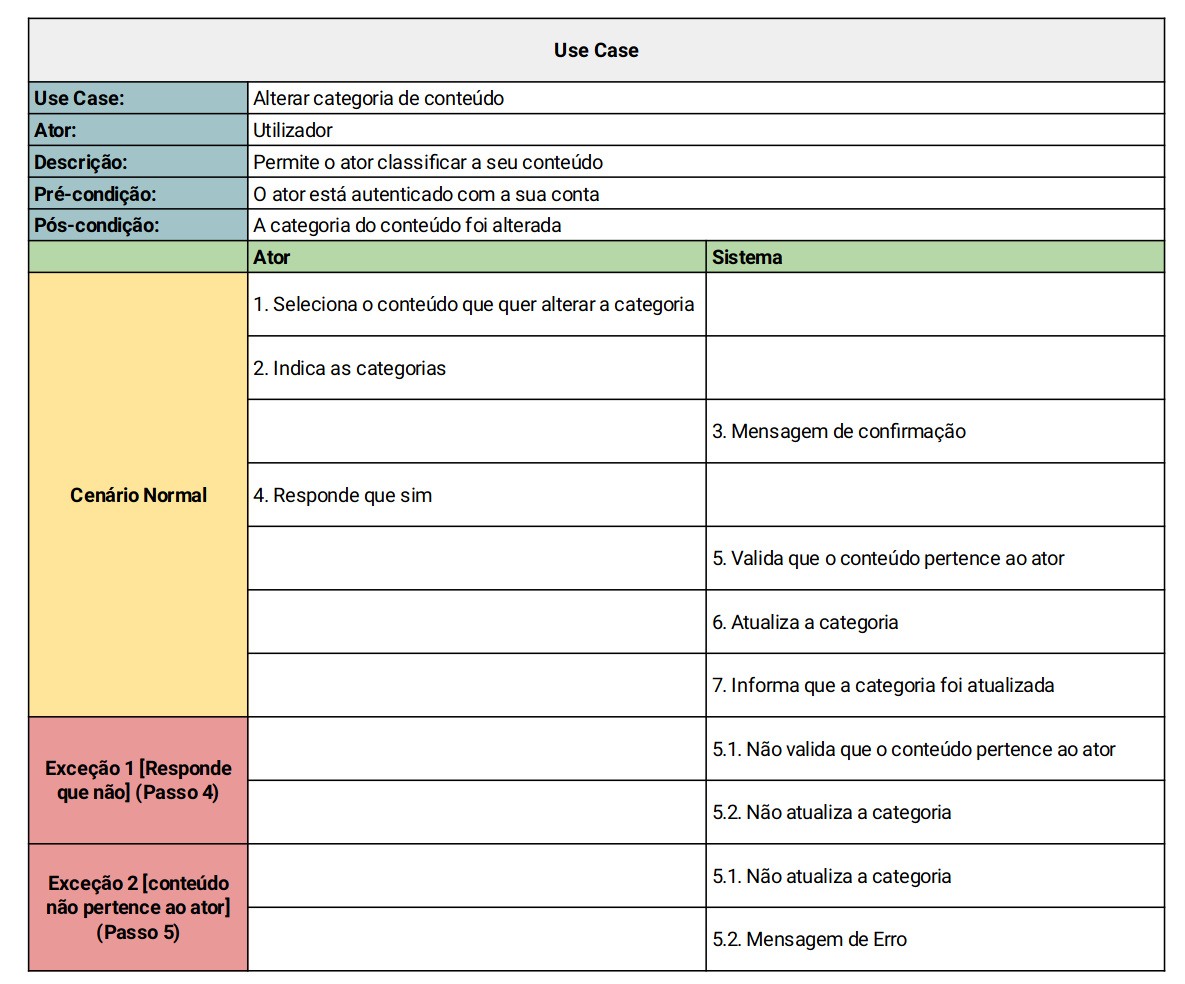
\includegraphics[width=\textwidth]{images/Classificar.png}  
    \caption{Especificação do \emph{Use Case} Classificar}
\end{figure}

\subsection{Criar Biblioteca}

\begin{figure}[H]
	\centering 
    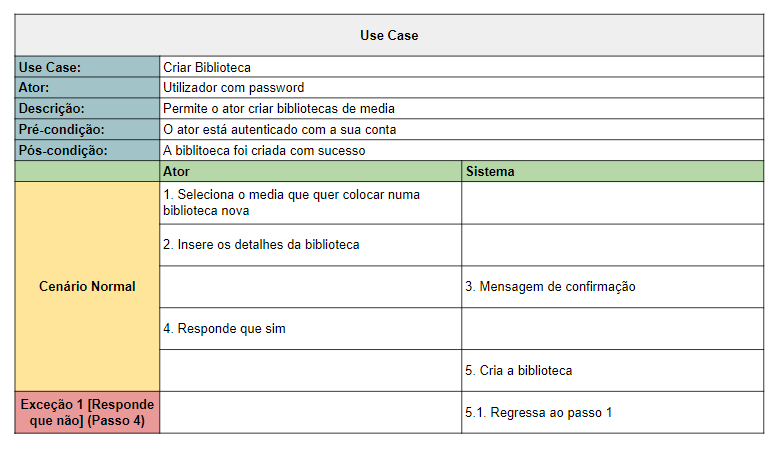
\includegraphics[width=\textwidth]{images/Criar_Biblioteca.png}  
    \caption{Especificação do \emph{Use Case} Criar Biblioteca}
\end{figure}

\subsection{Eliminar Biblioteca}

\begin{figure}[H]
	\centering 
    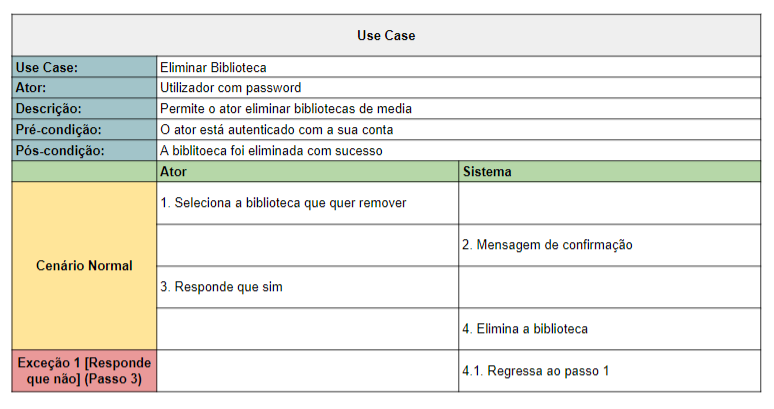
\includegraphics[width=\textwidth]{images/Eliminar_Biblioteca.png}  
    \caption{Especificação do \emph{Use Case} Eliminar Biblioteca}
\end{figure}

\subsection{Adicionar amigo}

\begin{figure}[H]
	\centering 
    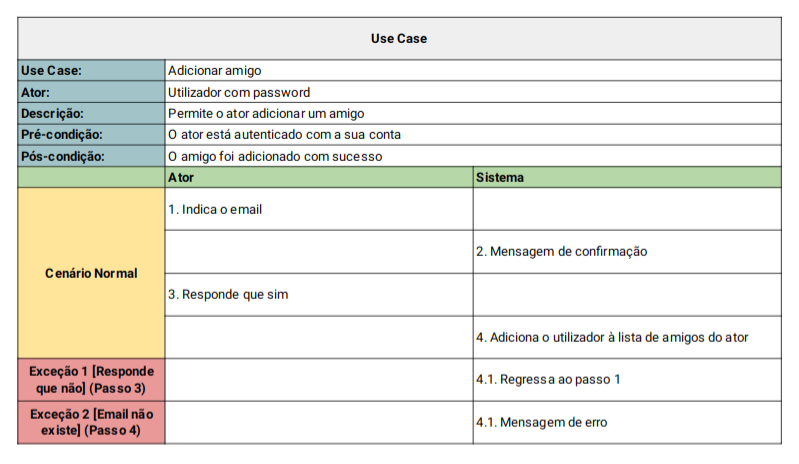
\includegraphics[width=\textwidth]{images/Adicionar_Amigo.png}  
    \caption{Especificação do \emph{Use Case} Adicionar amigo}
\end{figure}

\subsection{Remover amigo}

\begin{figure}[H]
	\centering 
    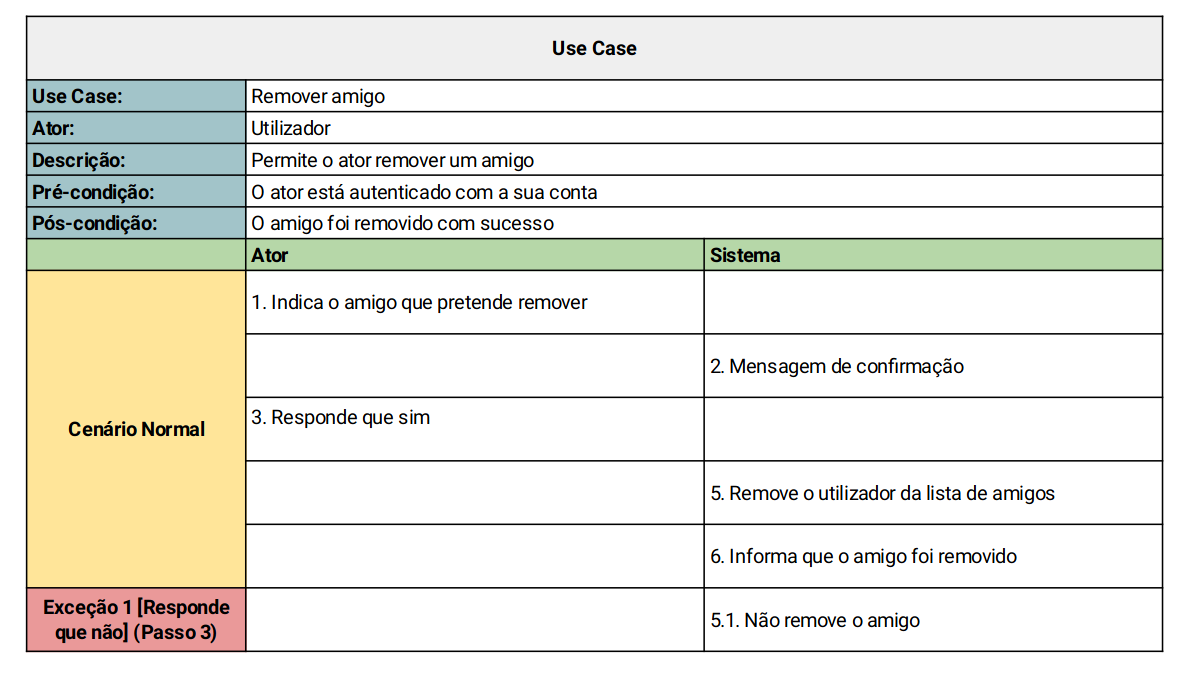
\includegraphics[width=\textwidth]{images/Remover_Amigo.png}  
    \caption{Especificação do \emph{Use Case} Remover amigo}
\end{figure}

\subsection{Criar Conta}

\begin{figure}[H]
	\centering 
    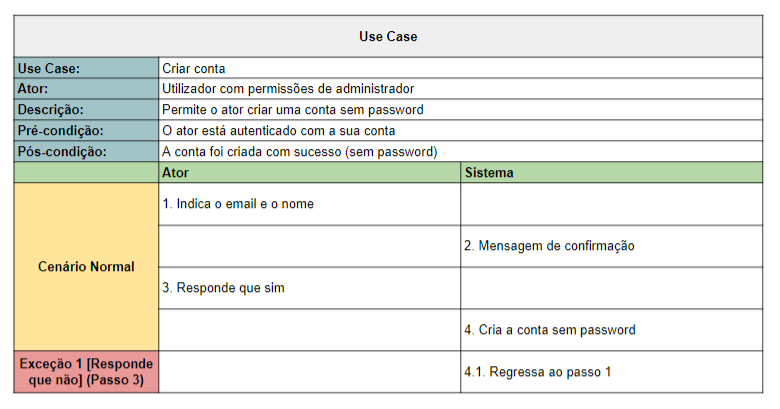
\includegraphics[width=\textwidth]{images/Criar_Conta.png}  
    \caption{Especificação do \emph{Use Case} Criar conta}
\end{figure}

\subsection{Remover conta}

\begin{figure}[H]
	\centering 
    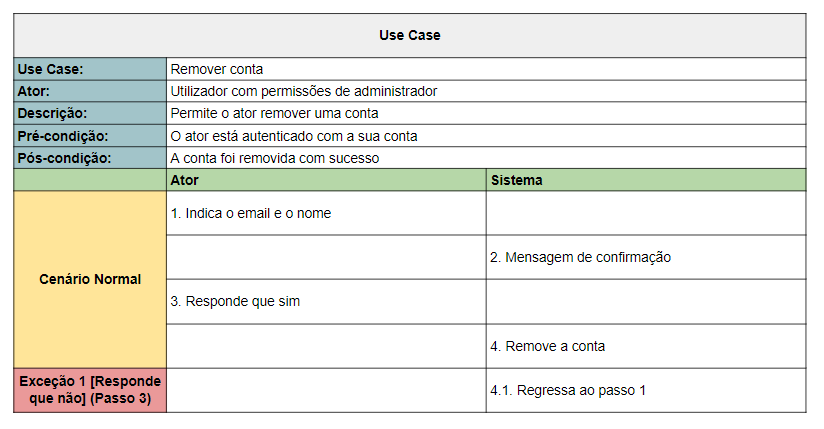
\includegraphics[width=\textwidth]{images/Remover_Conta.png}  
    \caption{Especificação do \emph{Use Case} Remover conta}
\end{figure}

\chapter{Mockups}

\textit{Mockups} é o nome dado aos protótipos de interface e como o próprio nome
indica é uma demonstração de como a aplicação final vai ser. O nosso foco enquanto 
se desenhava os protótipos foi a intuitividade mas mantendo uma aparência agradável

\section{Sem sessão iniciada}

\begin{figure}[H]
	\centering 
    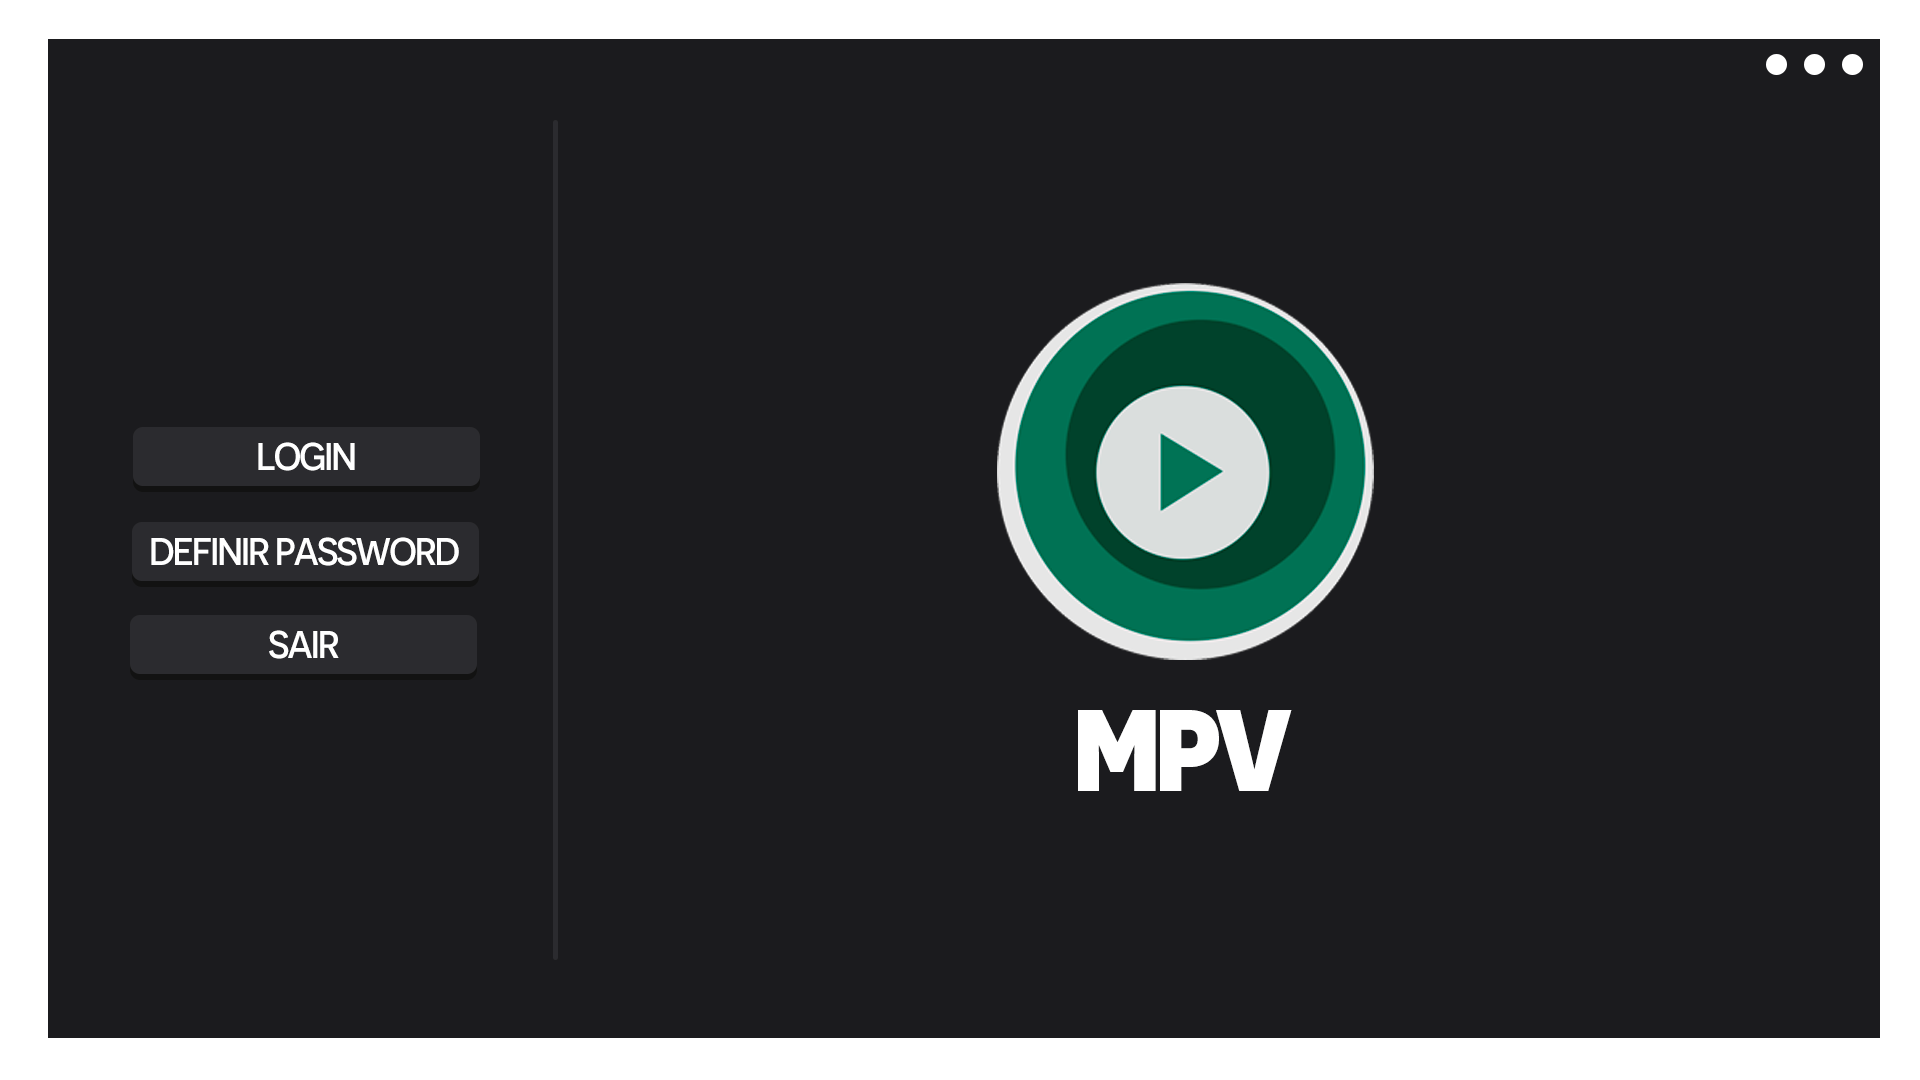
\includegraphics[width=\textwidth]{images/Inicio_Menu.png}  
    \caption{Menu inicial}
\end{figure}

\begin{figure}[H]
	\centering 
    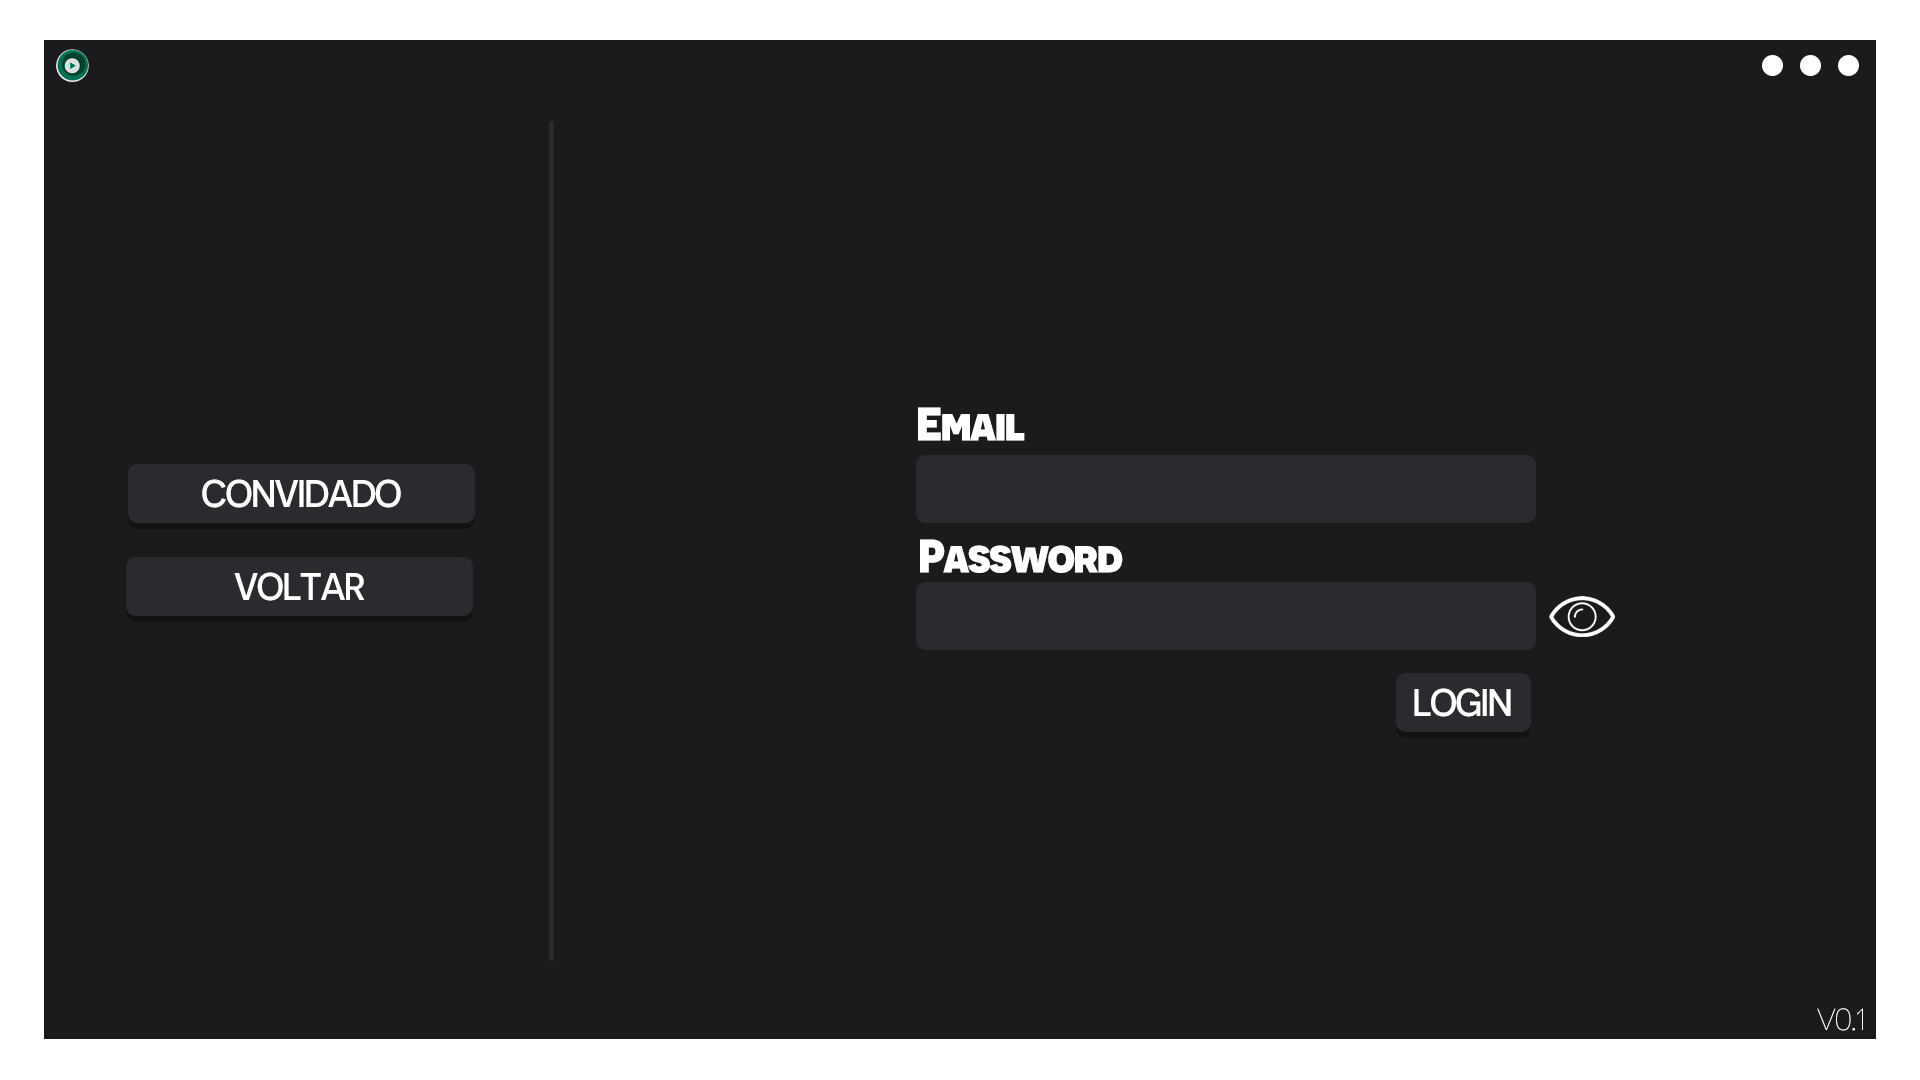
\includegraphics[width=\textwidth]{images/Login_Menu.png}  
    \caption{Login}
\end{figure}

\begin{figure}[H]
	\centering 
    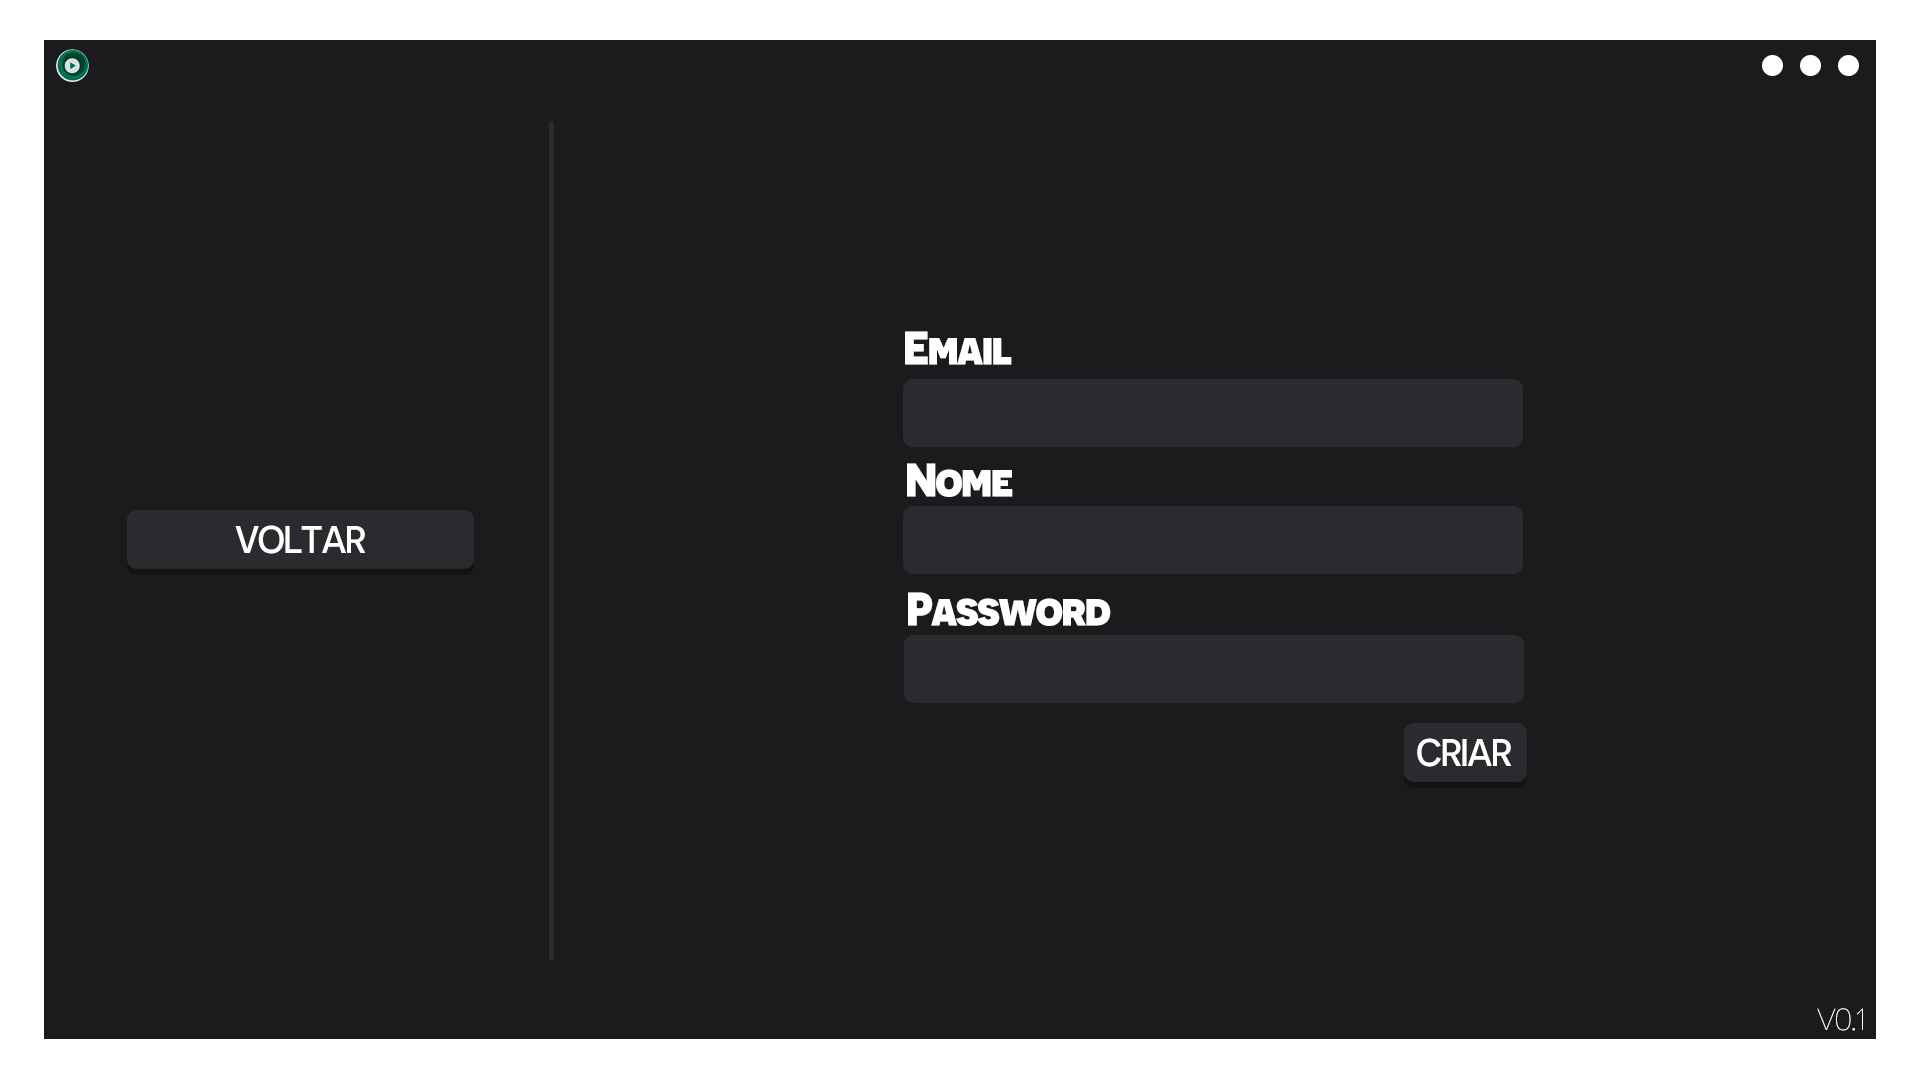
\includegraphics[width=\textwidth]{images/DefinirPassword_Menu.png}  
    \caption{Definir password para os utilizadores sem password a definirem}
\end{figure}

\begin{figure}[H]
	\centering 
    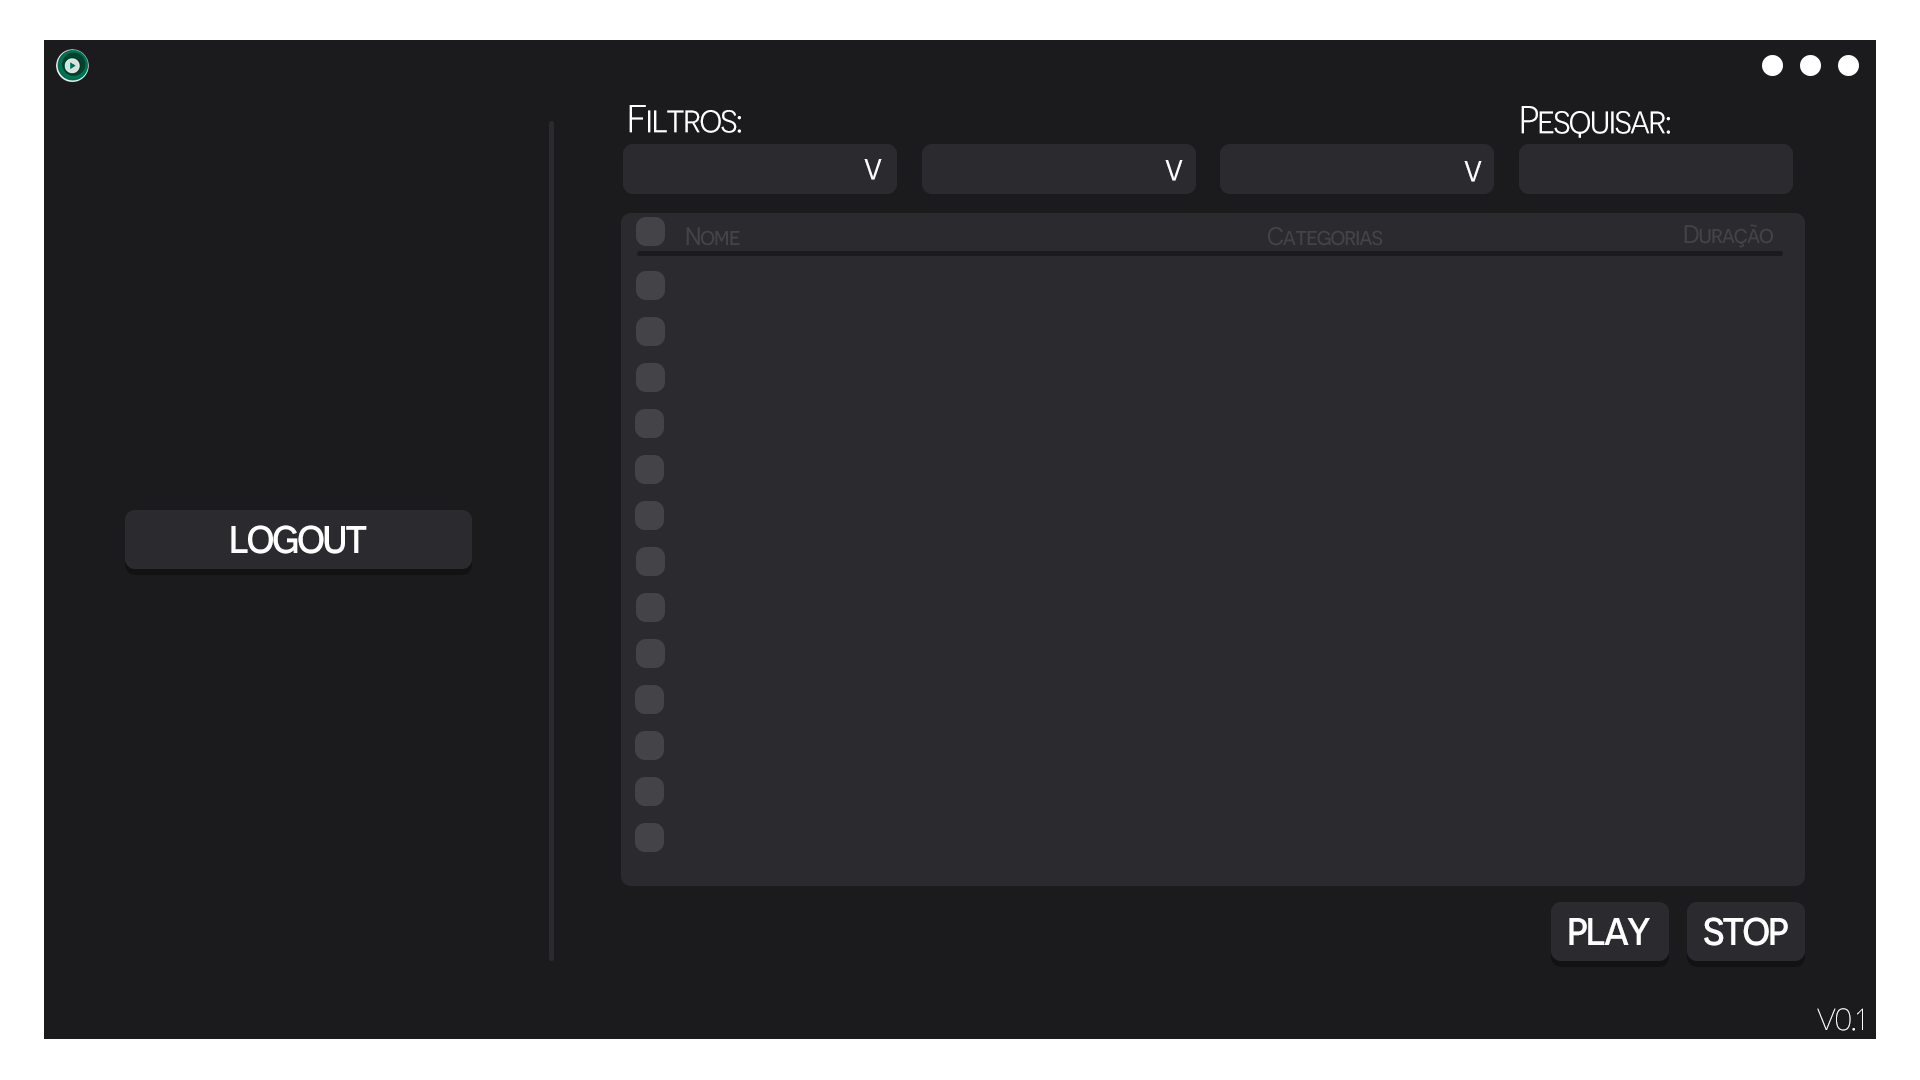
\includegraphics[width=\textwidth]{images/Principal_convidado_Menu.png}  
    \caption{Menu para um utilizador que entrou como convidado}
\end{figure}

\section{Com sessão iniciada}

\begin{figure}[H]
	\centering 
    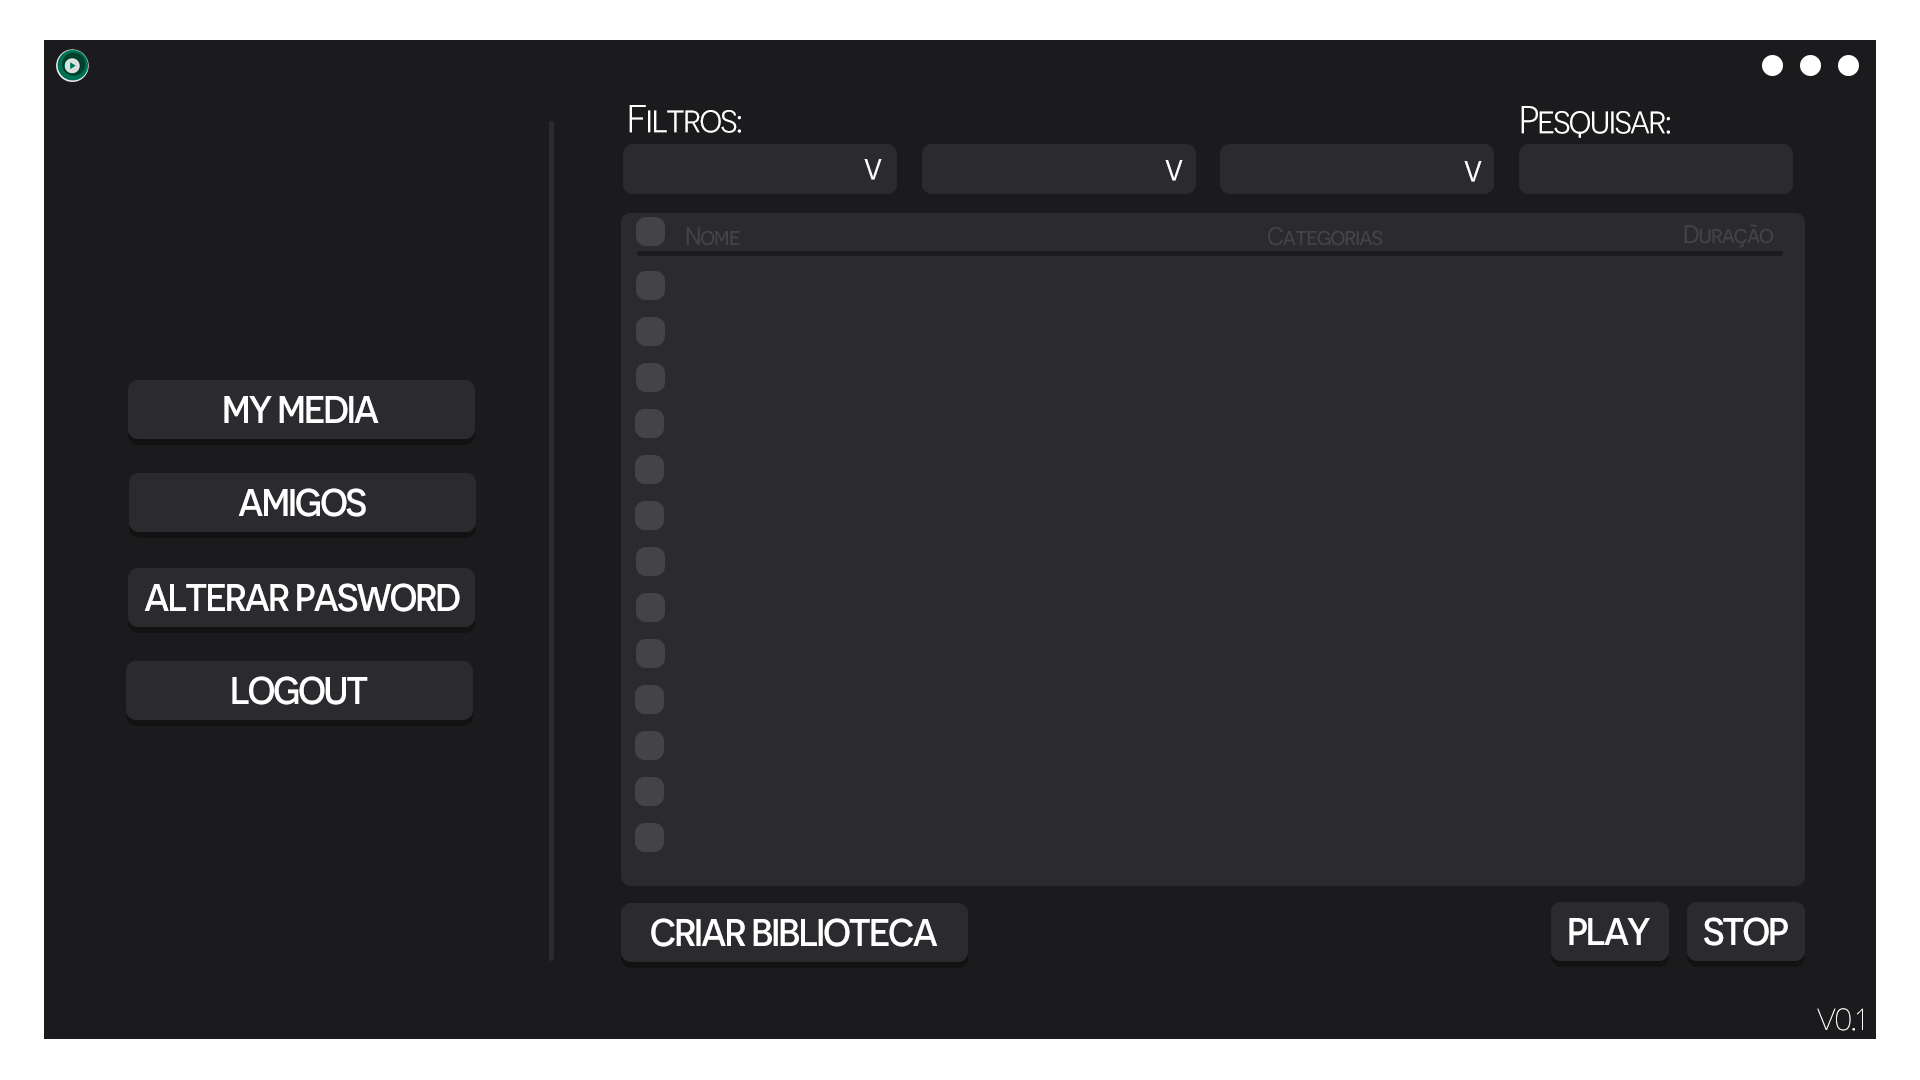
\includegraphics[width=\textwidth]{images/Principal_Menu.png}  
    \caption{Menu para um utilizador autenticado com password}
\end{figure}

\begin{figure}[H]
	\centering 
    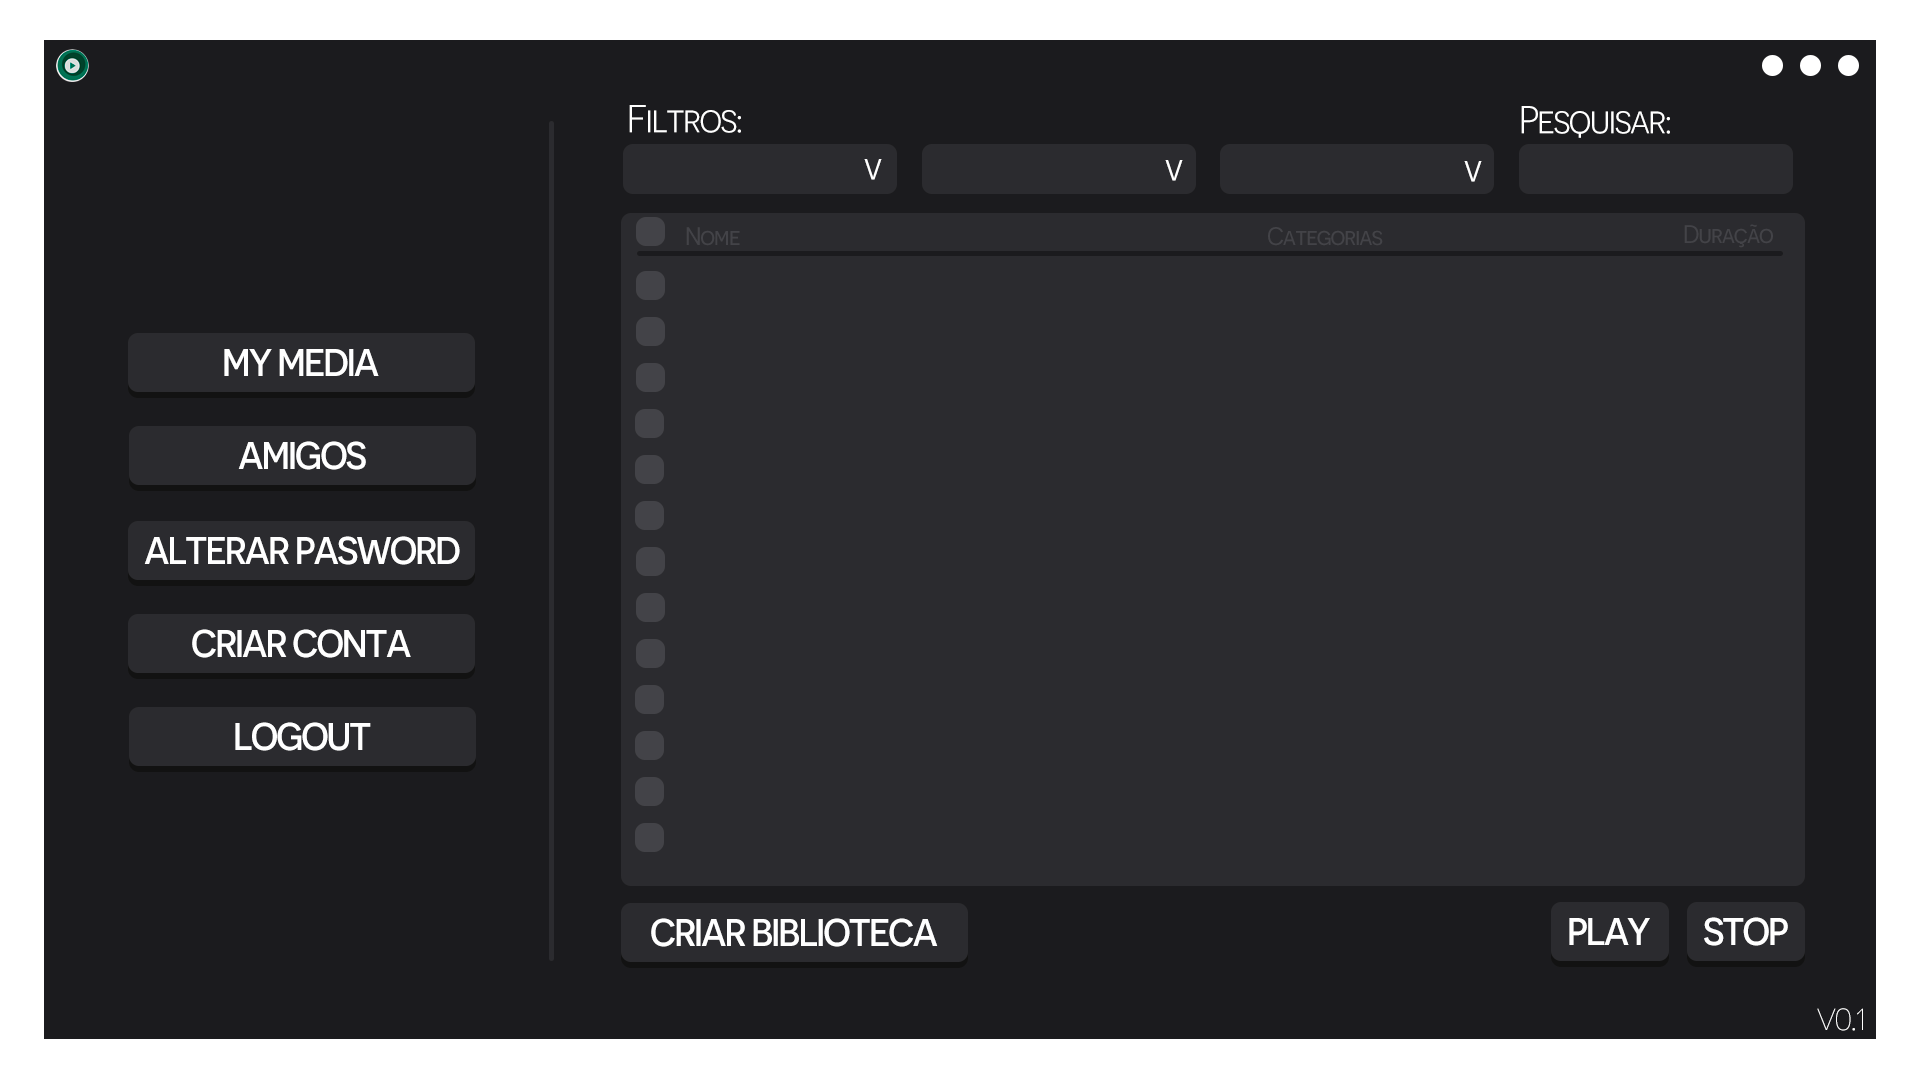
\includegraphics[width=\textwidth]{images/Principal_Admin_Menu.png}  
    \caption{Menu para um utilizador com permissões de administrador autenticado}
\end{figure}

\begin{figure}[H]
	\centering 
    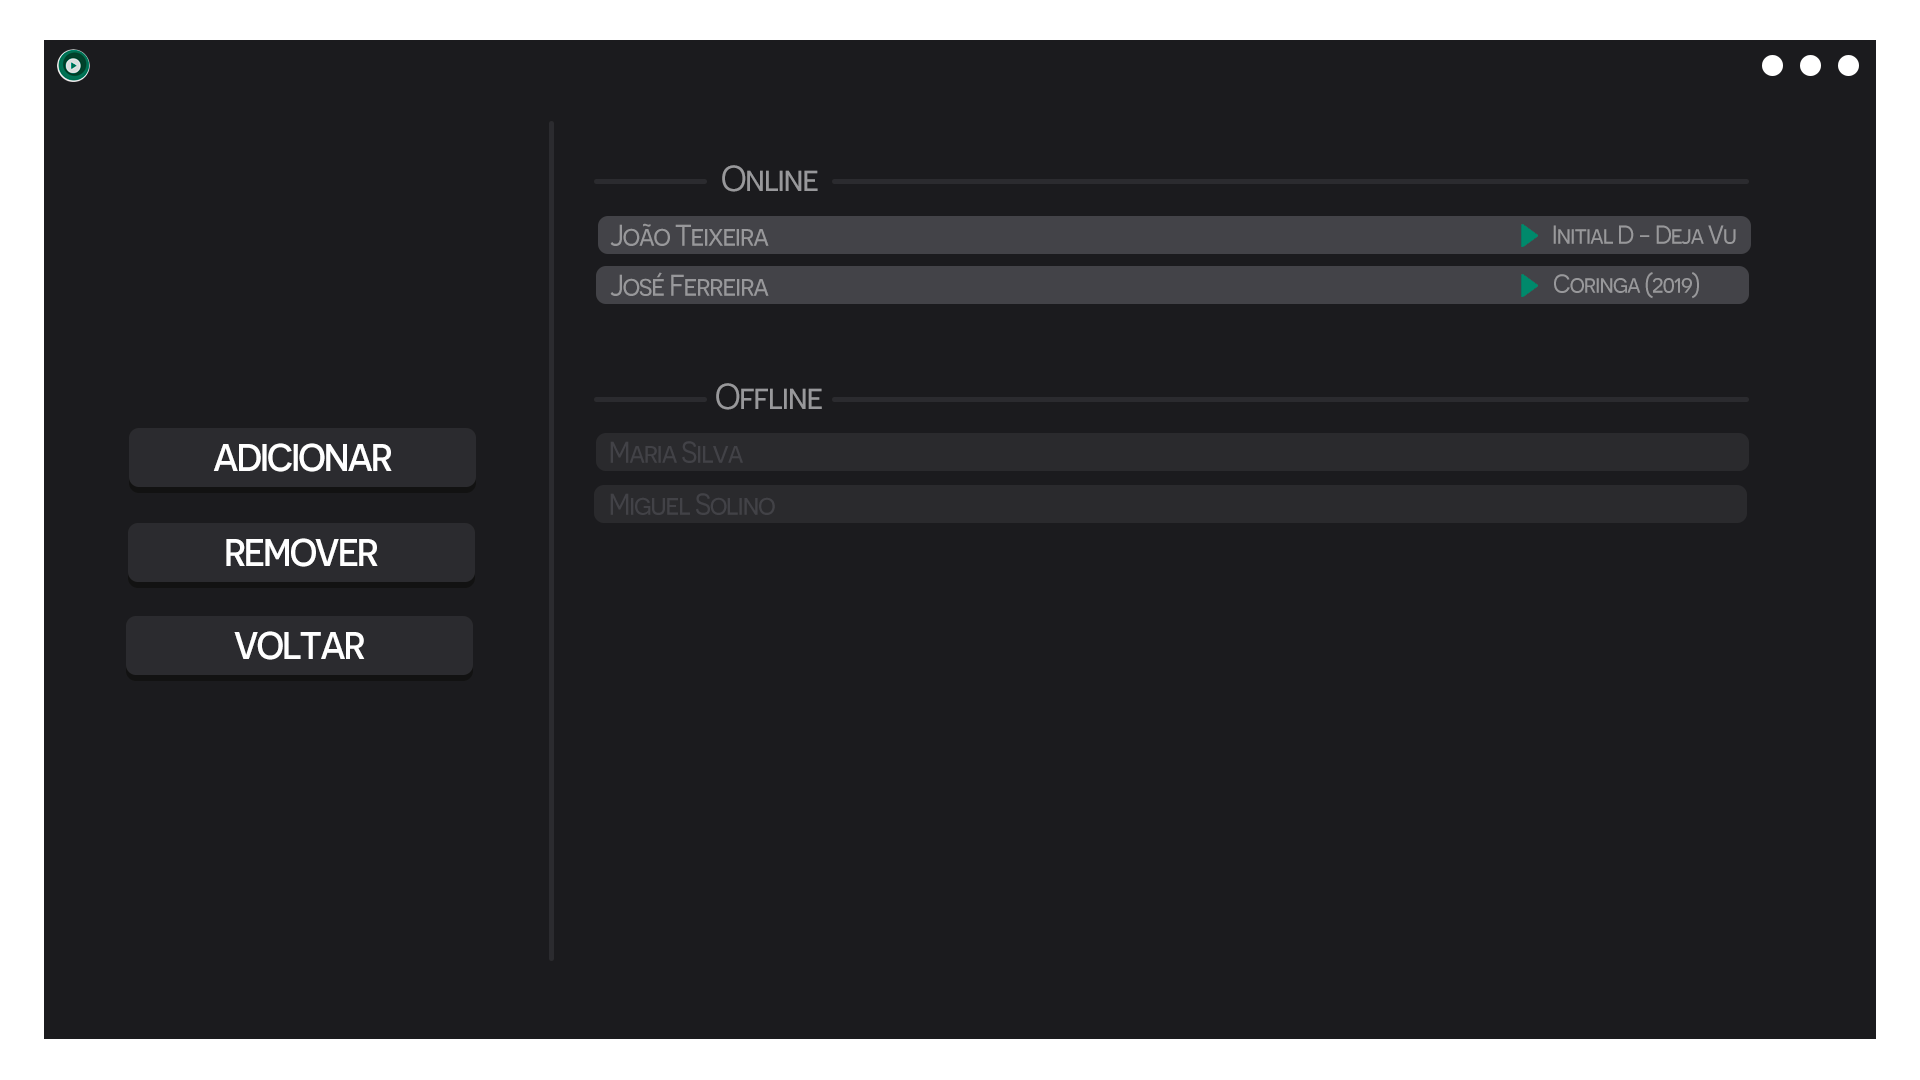
\includegraphics[width=\textwidth]{images/Amigos_Menu.png}  
    \caption{Menu com as amizades}
\end{figure}

\begin{figure}[H]
	\centering 
    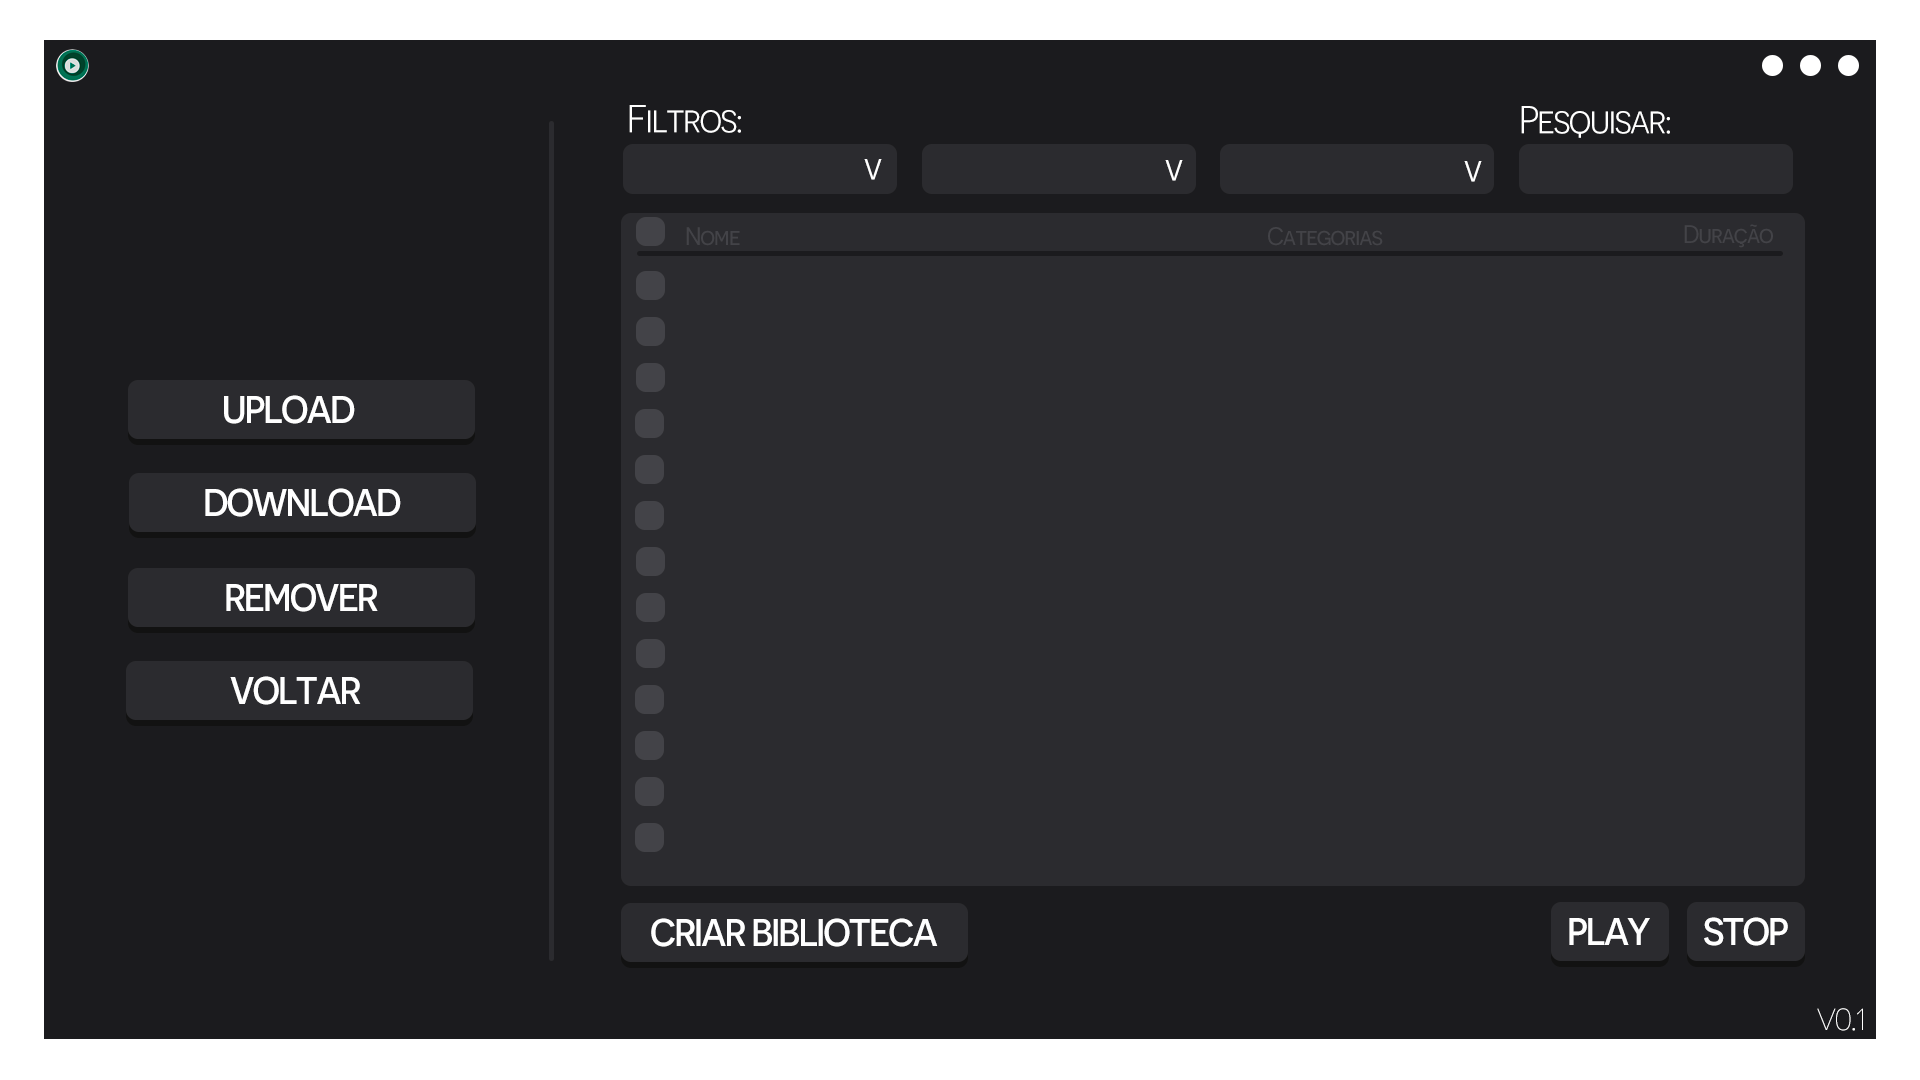
\includegraphics[width=\textwidth]{images/MyMedia_Menu.png}  
    \caption{Menu com a media do utilizador autenticado}
\end{figure}

\begin{figure}[H]
	\centering 
    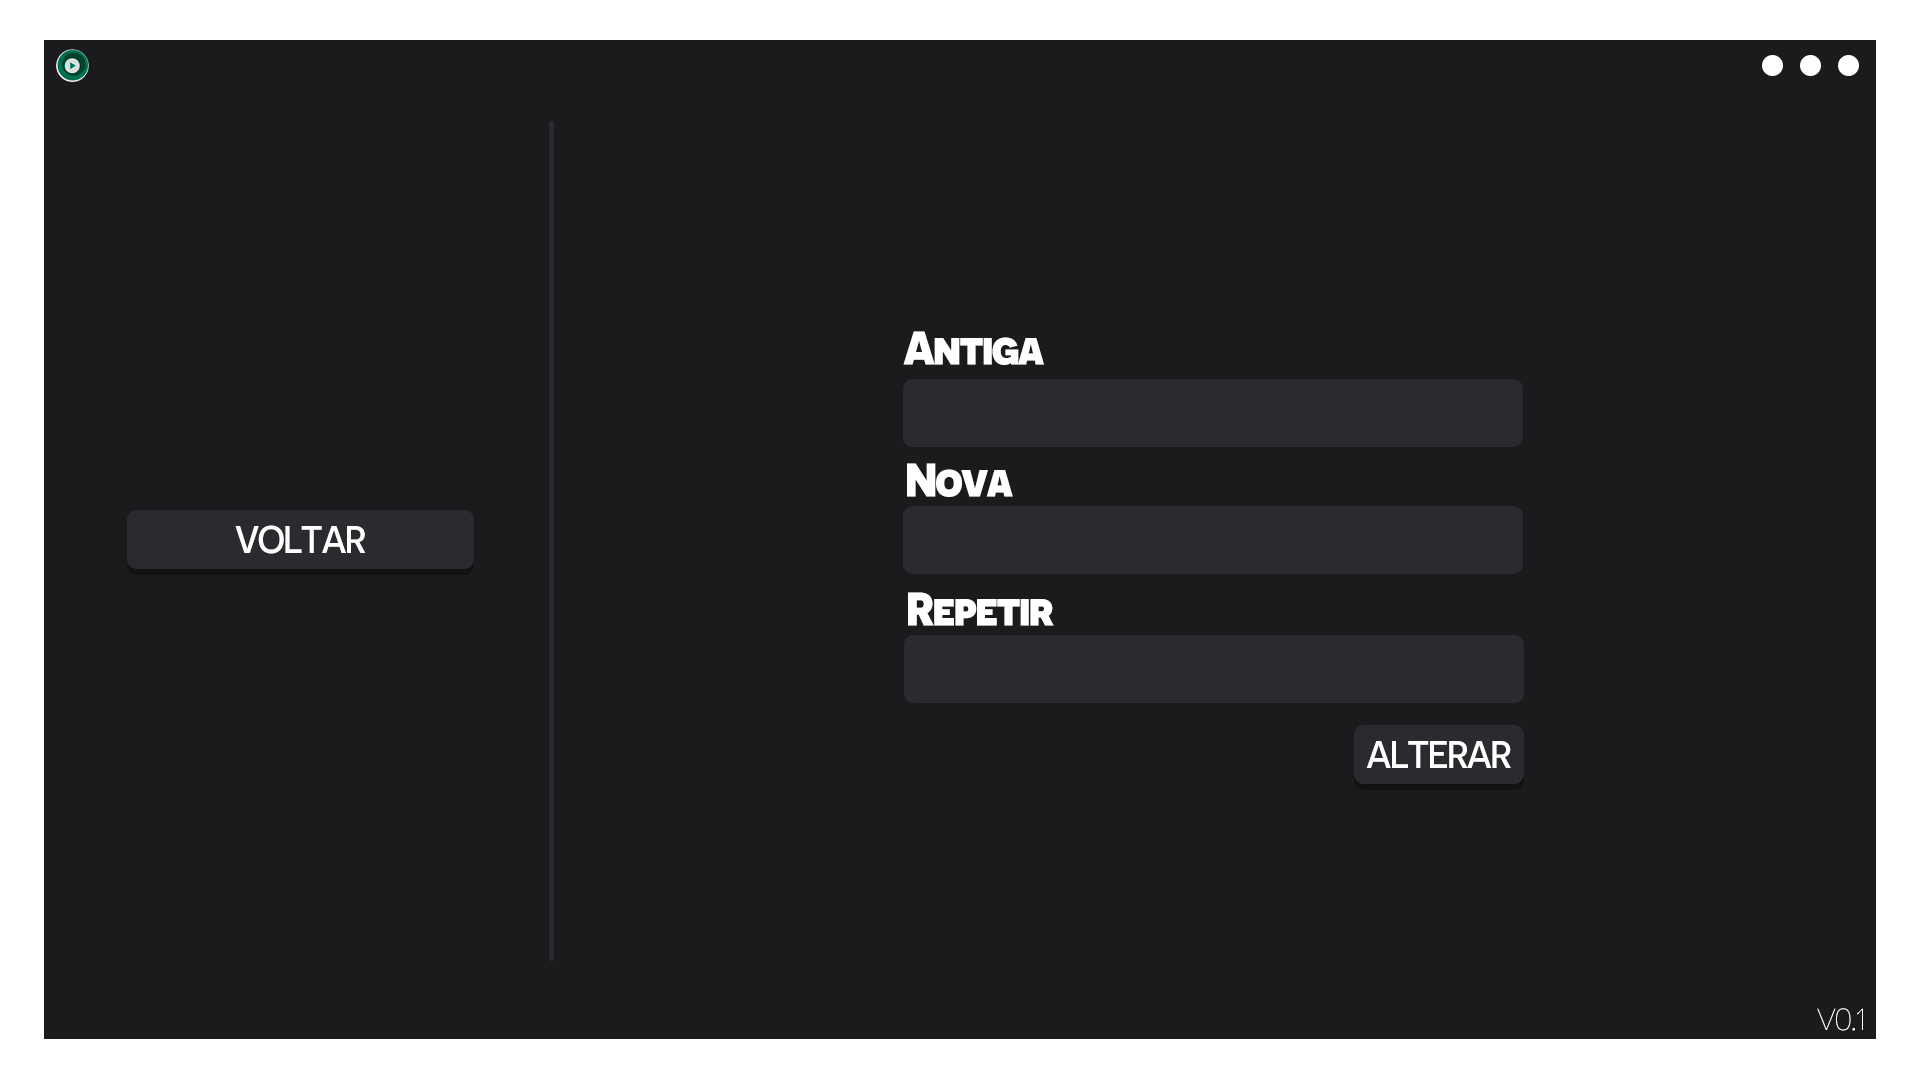
\includegraphics[width=\textwidth]{images/AlterarPassword_Menu.png}  
    \caption{Menu para alterar a password}
\end{figure}

\begin{figure}[H]
	\centering 
    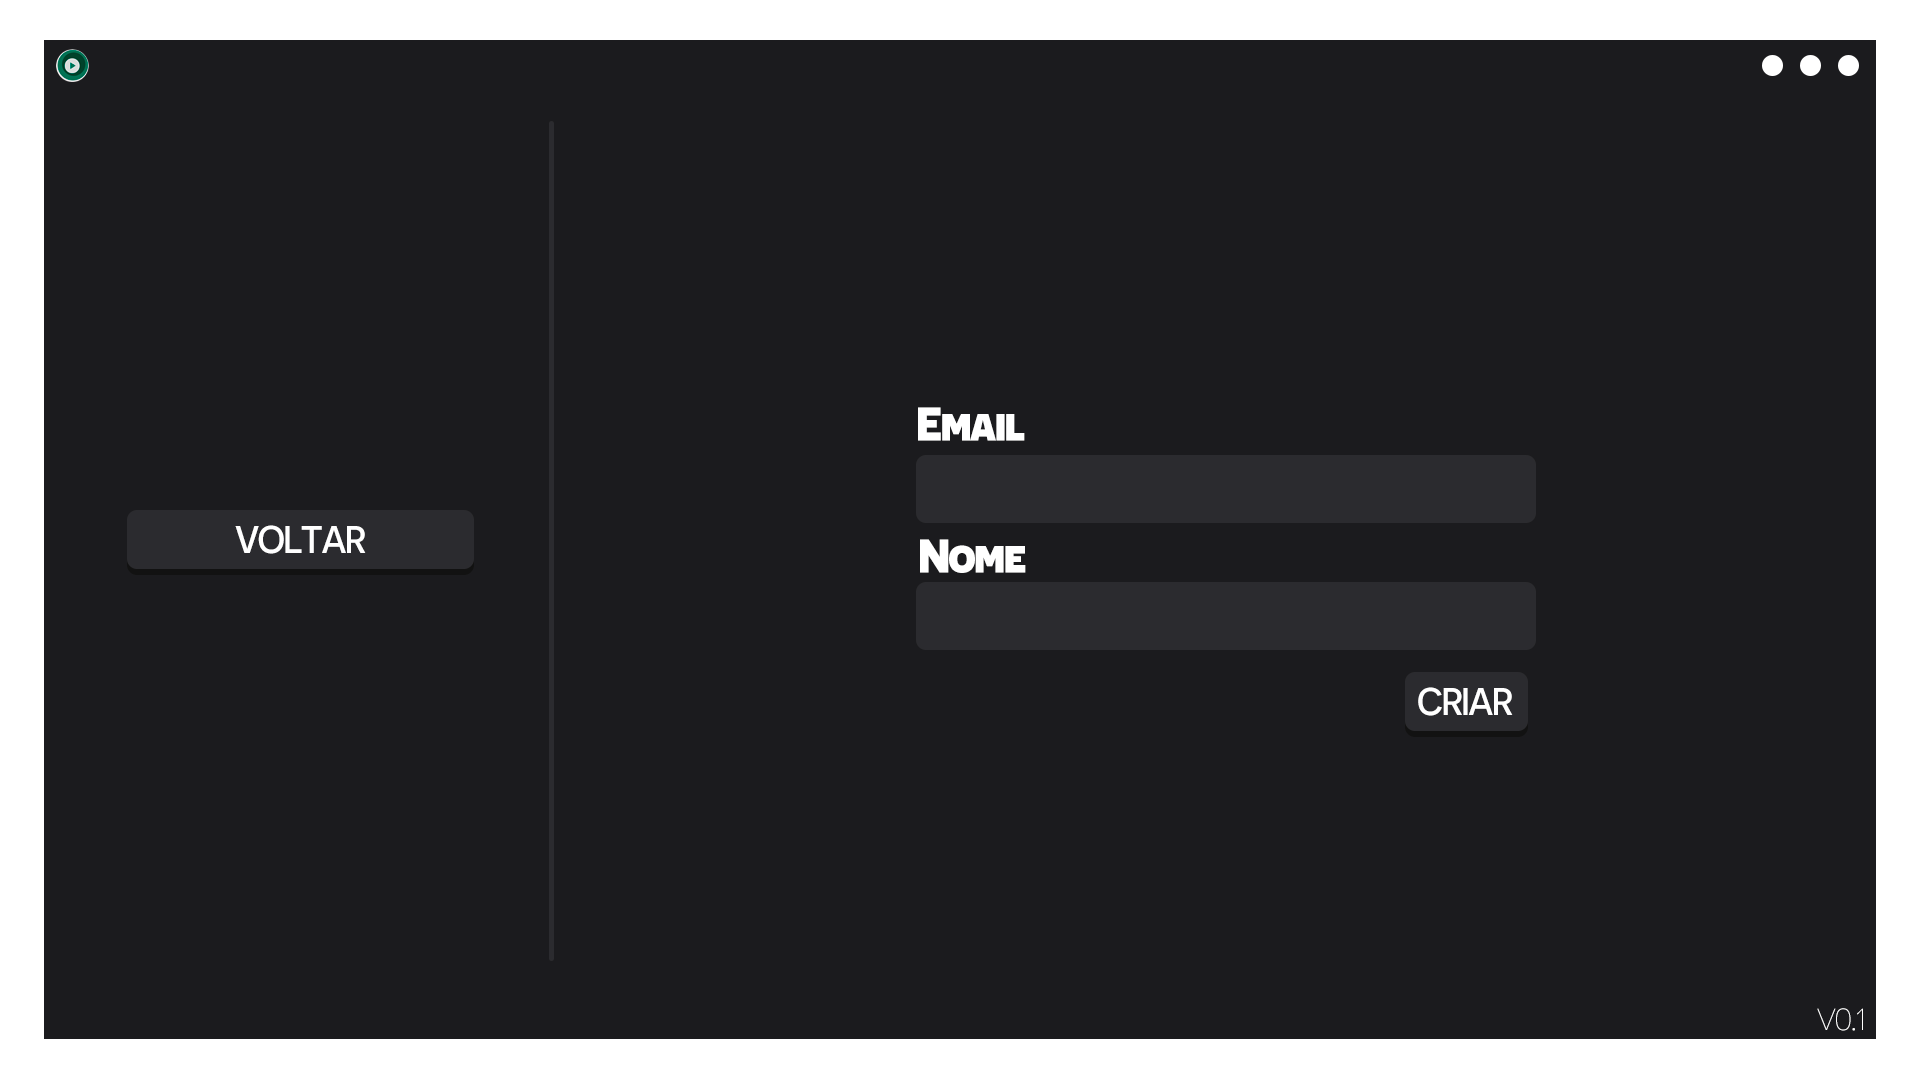
\includegraphics[width=\textwidth]{images/CriarConta_Menu.png}  
    \caption{Menu para utilizadores com permissões de administrador criarem contas sem password}
\end{figure}

\begin{figure}[H]
	\centering 
    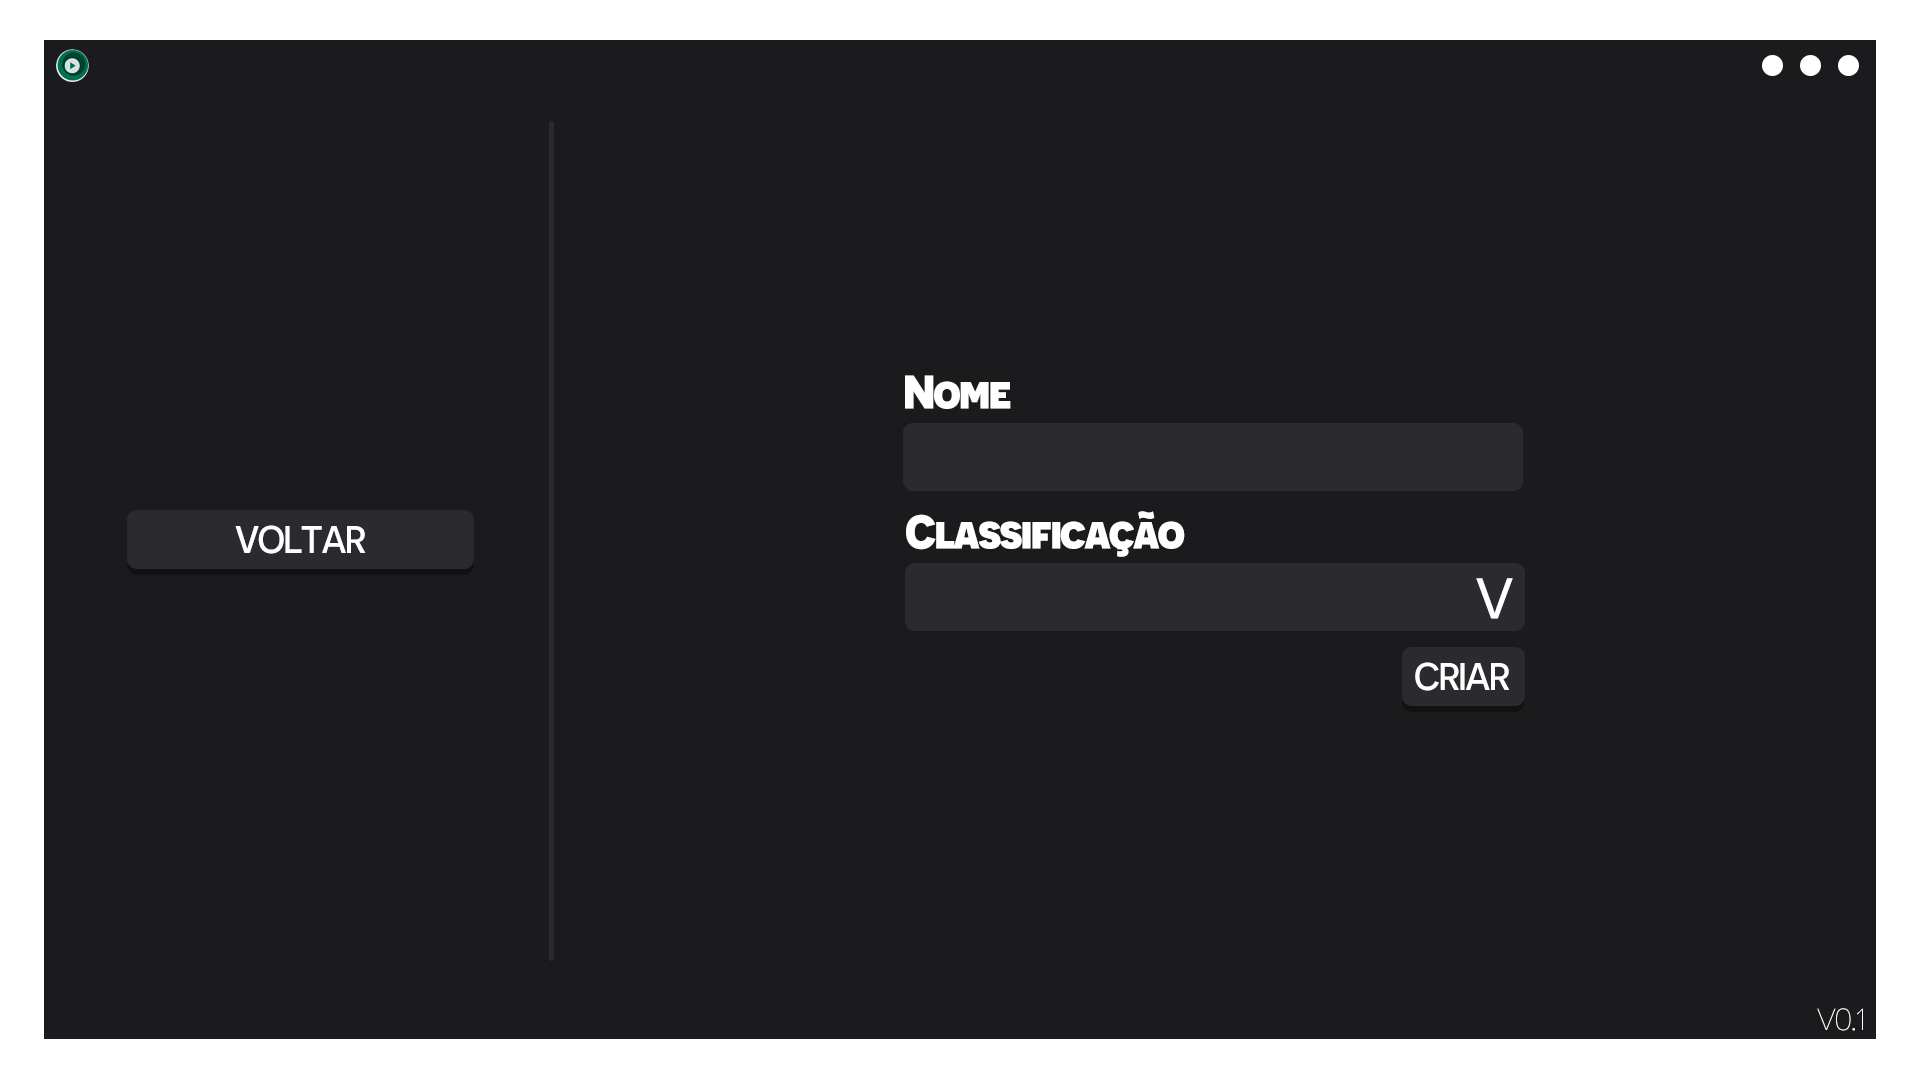
\includegraphics[width=\textwidth]{images/Criar_Biblioteca_Menu.png}  
    \caption{Menu para criar uma biblioteca}
\end{figure}

\begin{figure}[H]
	\centering 
    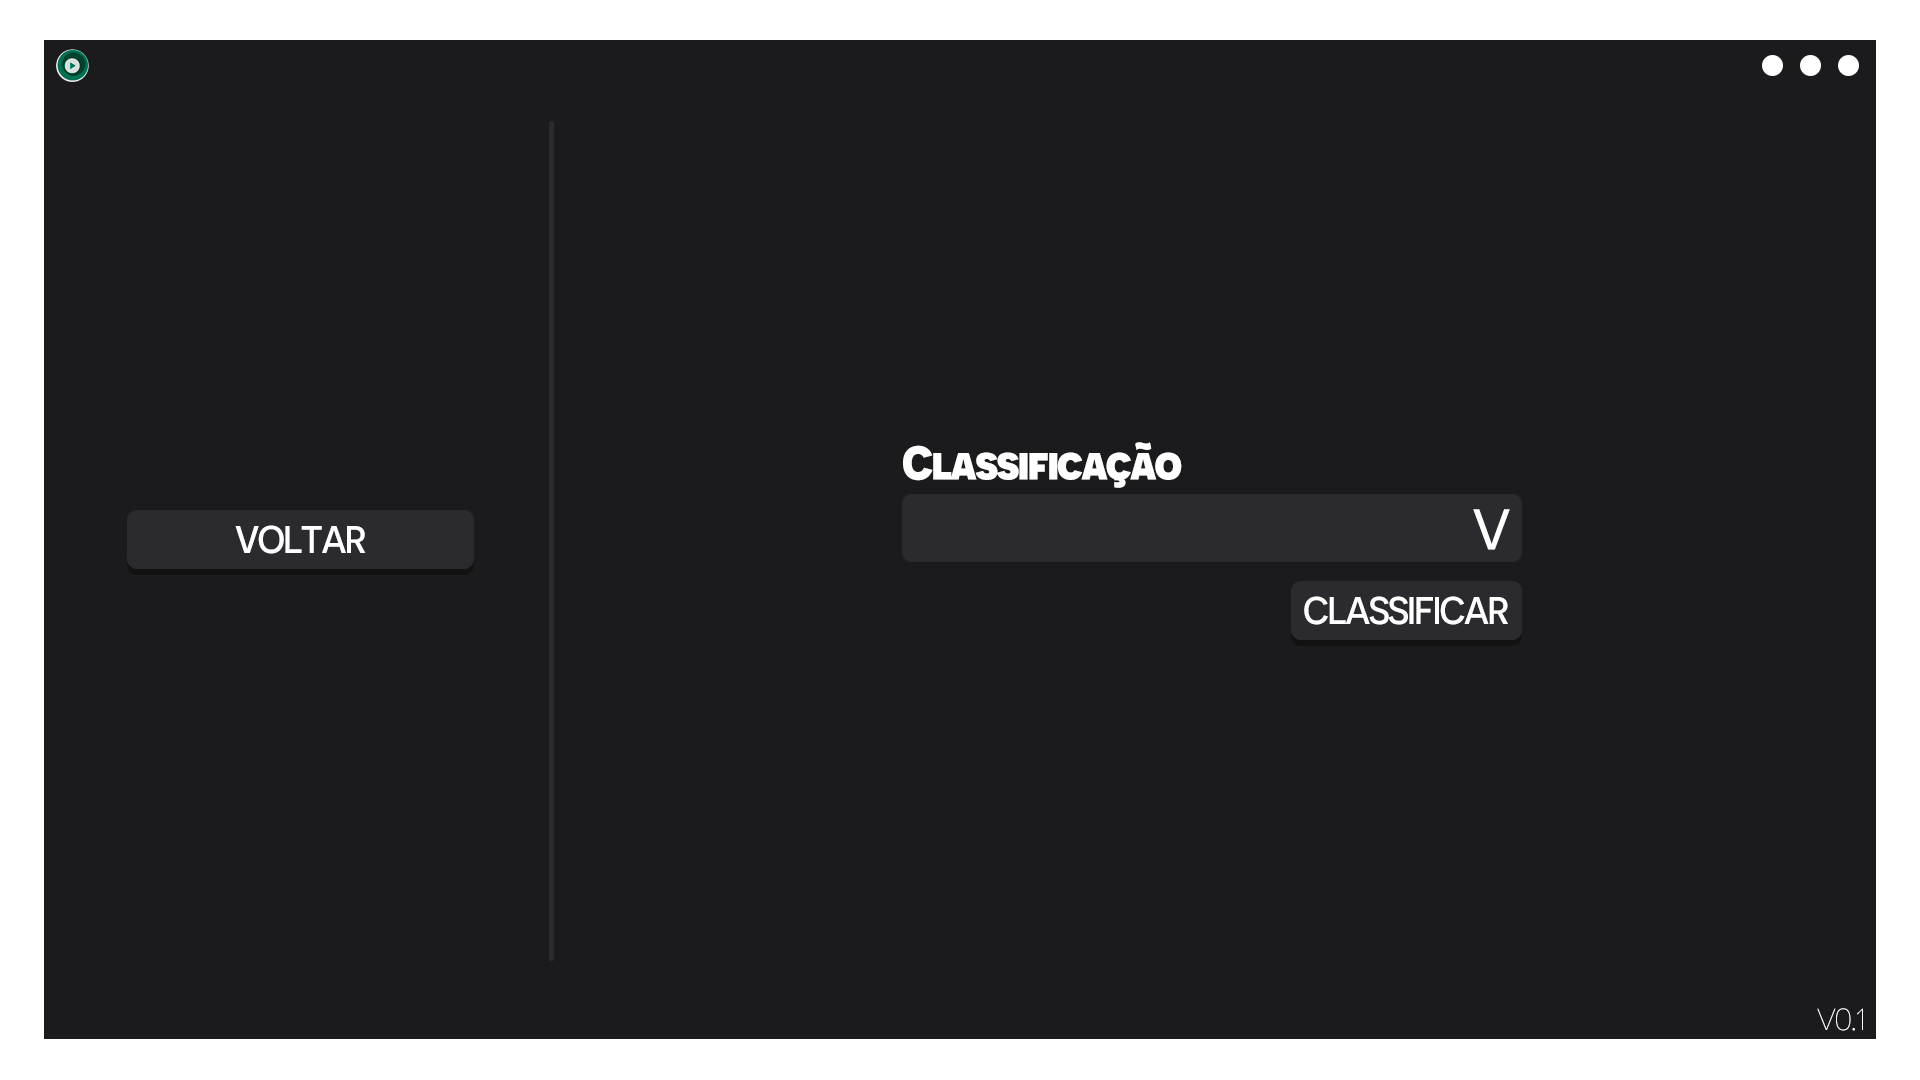
\includegraphics[width=\textwidth]{images/Classificar_Menu.png}  
    \caption{Menu para classificar um ou mais media}
\end{figure}


\end{document}
